\documentclass[a4paper, 12pt, BCOR10mm, DIV12, toc=bibliography, toc=listof, german]{scrbook}

% Preamble {{{
\usepackage[ngerman]{babel}
\usepackage[utf8]{inputenc}
\usepackage[T1]{fontenc}
\usepackage[pdftex]{graphicx}
\usepackage[%
	colorlinks=false,
	pdfborder={0 0 0},
]{hyperref}
\usepackage{epstopdf}
\usepackage[numbers]{natbib}
\usepackage{setspace}
\usepackage{amsmath, amsthm, amssymb}
\usepackage{scrpage2}
\usepackage{units}
\usepackage{listings}
\usepackage{color}
\usepackage{xcolor}

\definecolor{uniblue}{rgb}{0.062745,0.17647,0.34118}
\definecolor{tblue}{HTML}{204A87}
\definecolor{tgreen}{HTML}{4E9A06}
\definecolor{tred}{HTML}{CC0000}

\lstset{
	language=C,
	numbers=left,
	frame=single,
	basicstyle=\footnotesize,
	captionpos=b,
	breaklines=true,
	breakatwhitespace=false,
	keywordstyle=\color{tgreen},
	commentstyle=\color{tblue},
	stringstyle=\color{tred}
}

\setcounter{secnumdepth}{3}
\setcounter{tocdepth}{3}

% Titlepage {{{
\usepackage[absolute]{textpos}

\newlength{\TitleMargin}
\newlength{\TitleWidth}

\setlength{\TitleMargin}{2cm}
\setlength{\TitleWidth}{\paperwidth}
\addtolength{\TitleWidth}{-\TitleMargin}
\addtolength{\TitleWidth}{-\TitleMargin}


\newcommand{\TitleUni}{Universität Potsdam}
\newcommand{\TitleInstitut}{Mathematisch-Naturwissenschaftliche Fakultät\\Institut für Informatik}
\newcommand{\TitleTitel}{Selbst-adaptive Lastverteilung für DNS-Cluster}
\newcommand{\TitleTyp}{Masterarbeit}
\newcommand{\TitleAutor}{Sebastian Menski}
\newcommand{\TitleBetreuerText}{Betreuer}
\newcommand{\TitleBetreuer}{Prof. Dr. Bettina Schnor\\ &M.Sc. Jörg Zinke}
\newcommand{\TitleAbschlussText}{zur Erlangung des akademischen Grades\\Master of Science\\in Informatik}
\newcommand{\TitleOrt}{Potsdam}
\newcommand{\TitleDatum}{7. Juli 2012}
\hypersetup{
	pdfauthor={Sebastian Menski},
	pdftitle={\TitleTitel},
}

\renewcommand{\maketitle}{
	\thispagestyle{empty}
	\begin{textblock*}{\TitleWidth}(\TitleMargin,\TitleMargin)
		~\hfill
\includegraphics[height=2.5cm]{images/uni-logo}\\[3mm]
		{\color{uniblue}\rule{\TitleWidth}{1mm}}\\[5mm]
		{
			\centering
			\sffamily\Large
			{\LARGE\TitleUni}\\[0.5\baselineskip]
			{\large\TitleInstitut}\\[5\baselineskip]
			{\Huge\TitleTitel}\\[3\baselineskip]

			{\TitleTyp}\\
			\TitleAbschlussText\\[3\baselineskip]

			\TitleAutor\\[3\baselineskip]
			\begin{tabular}{rl}
				\TitleBetreuerText: & \TitleBetreuer
			\end{tabular}\\[2\baselineskip]
			\TitleOrt, \TitleDatum\par
		}
	\end{textblock*}
	~\clearpage
}

\def \dns {Domain Name System (DNS)}

% Titlepage }}}

% Preamble }}}


\begin{document}
	 % Frontmatter {{{
	\frontmatter
	\maketitle{}
	\tableofcontents{}
	% Frontmatter }}}

	% Mainmatter {{{
	\onehalfspacing{}
	\mainmatter
	\pagestyle{scrheadings}

	\chapter{Einleitung} % {{{
	\label{cha:einleitung}

		Das \dns{} \cite{rfc1034, rfc1035} ist eine fundamentale Komponente des heutigen Internets.  Es
		ermöglicht eine Abbildung von Domain-Namen auf sogenannte IP\footnote{Das Internet Protocol (IP)
		\cite{rfc791} ist eines der wichtigsten Netzwerkprotokolle der TCP/IP-Suite
		\cite{stevens1994}. Es dient der Vermittlung von Daten-Paketen in einem Netzwerk, um dies zu
		ermöglichen erhält jeder Netzwerkteilnehmer eine eindeutige IP-Adresse.}-Adressen. Ein
		Domain-Name ist eine Zeichenkette, diese können sich Menschen leichter merken als eine
		Zahlenfolge.  Computersysteme hingegen können besser und schneller mit Zahlen als mit
		Zeichenketten arbeiten.  Daher ist diese Abbildung eine wichtige Voraussetzung für die einfache
		und schnelle Nutzung eines Netzwerks, im Besonderen des Internets. Bei jedem Aufruf einer
		Website oder dem Verschicken einer E-Mail, bei dem der Nutzer einen Domain-Namen nutzt, wird
		eine Abfrage an einen Server im DNS gestellt. Die darauffolgende Antwort, ist die dem
		Domain-Name zugeordnete IP-Adresse. Diese IP-Adresse wird dann vom Computersystem genutzt um
		eine Verbindung zum Ziel aufzubauen. Dieser Zusammenhang verdeutlicht bereits die Wichtigkeit
		des DNS, denn ohne dieses System müsste jeder Nutzer eines Netzwerks die benötigten IP-Adressen
		selber kennen. Dies ist vielleicht für ein kleines privates Netzwerk durchaus möglich, in
		Anbetracht der Größe des heutigen Internets jedoch	kaum vorstellbar. Aus diesem Grund ist ein
		stabiles System mit schnellen Antwortzeiten unerlässlich.

		Die Informationen im DNS werden dezentral gespeichert. Sie werden in einer verteilten,
		baumartigen Struktur gespeichert (siehe Abbildung \ref{fig:tree}). Dabei können verschiedene
		Server, die einzelnen Knoten des Baums und die dazugehörigen Informationen verwalten. Diese
		Server werden im Folgenden DNS-Server oder Nameserver genannten und haben die Aufgabe Fragen an
		das DNS zu beantworten. Aus der Struktur, des in Abbildung \ref{fig:tree} dargestellten Baums, ist
		zu erkennen, dass die kritischste Infrastruktur in den ersten beiden Ebenen des Baums existiert.
		Dabei handelt es sich um den Root-Server und alle Server der Top-Level-Domains (TLDs). Diese
		beiden Ebenen stellen die am häufigsten frequentierten Nameserver des DNS bereit, denn die Baumstruktur
		des DNS bedeutet, dass ein Knoten bzw. DNS-Server nur Informationen über den von ihm ausgehenden
		Teilbaum besitzt. Somit ist verständlich, dass die größte Menge an Informationen, beim Root-Server
		und den TLDs liegt.

		\begin{figure}
			\centering
			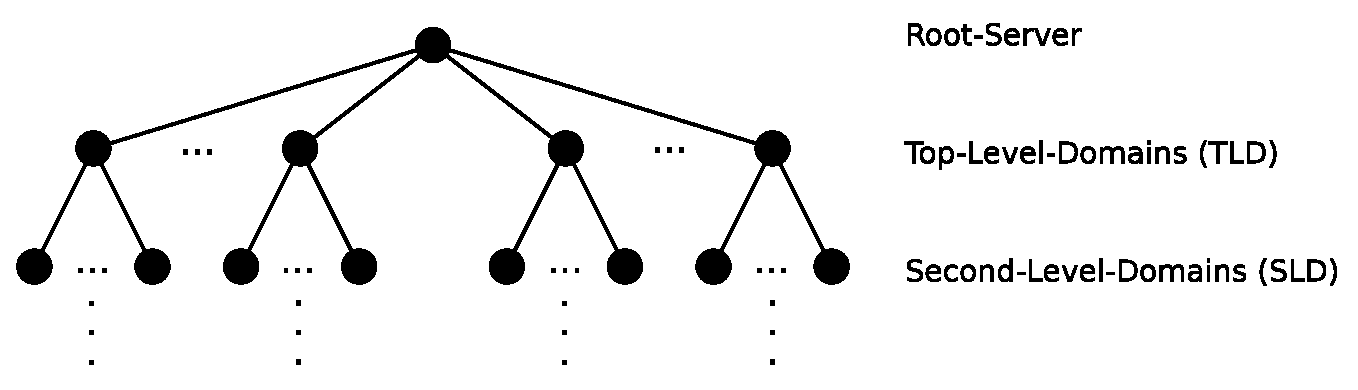
\includegraphics[width=\textwidth]{images/tree}
			\caption{Baumstruktur des \dns{}}
			\label{fig:tree}
		\end{figure}

		Ausfallsicherheit, ständige Verfügbarkeit und kurze Antwortzeiten sind Anforderungen, welche
		auch von vielen anderen Netzwerk-Diensten gefordert sind. Um diese Anforderungen zu erfüllen,
		gibt es das Konzept der Lastverteilung. Dabei wird eine hohe Last auf einer Ressource dadurch
		verringert, dass die Gesamtlast auf mehrere identische Ressourcen verteilt wird. Somit ist die
		Last je Ressource geringer und besser handhabbar. Dieses Konzept findet allgemein in Netzwerken
		und bei Server-Systemen Anwendung \cite{bourke2001, kopparapu2002}. Aber auch speziellere
		Anwendungsgebiete wie die Verteilung von Last auf Webservern sind besonders interessant für
		Websites mit hohen Lastanforderungen \cite{meplho2012}. Hierbei wird die anfallende Last auf ein
		Cluster aus Backend-Servern verteilt, dabei stellt jeder der sogenannten Backend-Server die
		gleiche Anwendung bereit. Die Aufgabe der Verteilung übernimmt dabei meist ein Lastverteiler,
		welcher vor den Backend-Servern in das Netzwerk eingefügt wird. Jede Anfrage wird somit durch
		den Lastverteiler geleitet, und dann von diesem an einen verfügbaren Backend-Server
		weitergeleitet. Diese allgemeinen Konzepte lassen sich ebenfalls für hohe Lastsituationen im DNS
		nutzen.

		Diese Arbeite beschäftigt sich mit dem Thema der Lastverteilung von DNS-Anfragen. Dazu wird ein
		bestehendes System \cite{zinke2007,scsczile2008,zinke2012,salbnet} zur selbst-adaptiven
		Lastverteilung von TCP-Anfragen erweitert, so dass es ebenfalls UDP-Anfragen verarbeiten kann.
		Dieses System ist in dem Sinne selbst-adaptive, dass der Lastverteiler keine eigenständigen
		Annahmen über die Last der Backend-Server trifft. Jeder Backend-Server ermittelt eigenständig
		eine Einschätzung der aktuellen Lastsituation. Diese wird dem Lastverteiler über Credits
		mitgeteilt. Dabei entspricht ein Credit einer weiteren Verbindung, welche von dem Server
		abgearbeitet werden kann. Somit passt sich der Lastverteiler, immer eigenständig an die aktuelle
		Lastsituation auf den Backend-Server an, ohne dass ein Administrator Einstellungen am
		Lastverteiler vornehmen muss.  Damit unterscheidet sich das System von anderen
		Lastverteilungs-Algorithmen, welche meist initial konfiguriert werden und danach kaum
		beeinflussbar sind. So kann auch eine fehlerhaft initiale Konfiguration nicht im laufenden
		Betrieb ausgebessert werden. Das selbst-adaptive System hingegen sollte sich an verschiedene
		Lastsituationen eigenständig anpassen.

		Das in \cite{zinke2007,scsczile2008} beschrieben System ist für TCP\footnote{Das Transmission
		Control Protocol (TCP) \cite{rfc793} ist ein zuverlässiges, verbindungsorientiertes und
		paketvermitteltes Transportprotokoll der TCP/IP-Suite \cite{stevens1994}. Es wird für
		Verbindungen eingesetzten, welche in dem Sinne verlässlich sind, dass verlorene Daten-Pakete
		erneut übertragen werden. Um dies zu realisieren ist allerdings ein gewisser Mehraufwand beim
		Verbindungsaufbau und -abbau nötig.  Bekanntestes Beispiel für TCP-Verbindungen stellen
		HTTP-Anfragen zum Abrufen und kommunizieren mit Websites dar.}-Anfragen implementiert. Und wurde
		anhand des Apache Webservers (httpd) \cite{httpd} getestet \cite{zinke2012}. Bei diesen Test
		wurden die Credits über ein InfiniBand \cite{infiniband,zinke2007} Netzwerk übertragen und direkt
		in den Speicher des Lastverteilers geschrieben\footnote{InfiniBand \cite{infiniband} ist eine
		Hochgeschwindigkeits-Übertragungstechnik, welche zusätzlich Remote Direct Memory Access (RDMA)
		unterstützt. Dies ermöglicht einen direkten Speicherzugriff auf einen über das Netzwerk verbunden
		Rechner.}. Durch diesen direkten Schreibzugriff, muss keine blockierende Kommunikation zwischen dem
		Lastverteiler und dem Backend-Server statt finden.

		Aufgabe dieser Arbeit ist es, dass bereits für TCP implementierte Verfahren ebenfalls für UDP zu
		implementieren. Das User Datagram Protocol (UDP) \cite{stevens1994, rfc768} ist ebenfalls ein
		paketvermitteltes Transportprotokoll aus der TCP/IP-Suite, jedoch im Gegensatz zum TCP
		verbindungslos und unzuverlässig. Das bedeutet der Verlust eines Daten-Pakets während der
		Übertragung wird nicht bemerkt und somit ist auch keine automatisch Wiederholung der Übertragung
		möglich. Diese Eigenschaft grenzt die Anwendungsfälle, in denen UDP sinnvoll einsätzbar ist
		bereits stark ein, allerdings entfällt durch diese Unzuverlässigkeit der Mehraufwand am Anfang
		und Ende einer zuverlässigen Verbindung, wie es zum Beispiel bei TCP der Fall ist. Da es sich
		bei DNS-Anfragen immer nur um eine Frage und eine Antwort handelt, welche schnell übertragen
		werden sollen, ist der Mehraufwand einer TCP-Verbindung nicht sinnvoll. Daher wird im
		Standardfall für DNS-Anfragen UDP genutzt. Dabei ist das allgemeine Vorgehen so, dass Anfragen,
		welche nicht in einem bestimmten Zeitraum beantwortet wurden, erneut gesendet werden. Diese
		Unterschiede zwischen TCP und UDP müssen bei der Erweiterung des bestehenden Systems beachtet
		werden.  Außerdem wird zur Übertragung der Credits, zwischen den Backend-Servern und dem
		Lastverteiler, eine TCP/IP-Verbindung über Ethernet genutzt. Dadurch soll verdeutlicht werden,
		dass dieses selbst-adaptive System auch über blockierende Kommunikation effizient ist.

		Die Arbeit ist in 8 Kapitel aufgeteilt. In Kapitel \ref{cha:grundlagen} werden die Grundlagen
		dieser Arbeit erklärt, dabei handelt es sich um das \dns{} und Lastverteilungsansätze, und es
		wird eine Einordnung dieser Arbeit in die vorgestellten Konzepte vorgenommen. Anschließend
		werden im Kapitel \ref{cha:arbeiten} einige Arbeiten aufgeführt, welche sich mit DNS-Clustern
		und Lastsituationen in eben diesen befassen. Das zu erweiternde System zur selbst-adaptiven
		Lastverteilung salbnet \cite{zinke2012,salbnet} wird in Kapitel \ref{cha:salbnet} beschrieben.
		In Kapitel \ref{cha:konzept} wird das Konzept der erarbeiteten Erweiterung und die dazugehörigen
		Vorüberlegungen aufgezeigt.  Darauf folgend ist in Kapitel \ref{cha:implementierung} die
		konkrete Umsetzung des vorher dargestellten Konzepts beschrieben.  Es wird hierbei auf
		Besonderheiten und Probleme bei der Implementation eingegangen.  Daran anschließend werden in
		Kapitel \ref{cha:messungen} die Ergebnisse einer Funktionsmessung und eine Einschätzung der
		Implementation vorgestellt. Am Ende dieser Arbeit folgt in Kapitel \ref{cha:zusammenfassung}
		eine Zusammenfassung, Einschätzung und Bewertung der erreichten Ziele und ein Ausblick auf
		mögliche Erweiterungen des Konzepts.

	% chapter Einleitung }}}

	\chapter{Grundlagen} % {{{
	\label{cha:grundlagen}

		Dieses Kapitel soll eine Einführung in die Verfahren und Techniken geben, die dieser Arbeit
		zugrundeliegen.  Dazu wird zu Beginn des Kapitels in Abschnitt \ref{sec:dns} auf die Entstehung,
		Bedeutung und Funktionsweise des \dns{} eingegangen. Außerdem werden Softwaresysteme
		vorgestellt, welche zum Betreiben eines DNS-Servers geeignet sind. Daran anschließend soll in
		Abschnitt \ref{sec:lastverteilung} ein Überblick über bestehende Konzepte und Praktiken der
		allgemeinen Lastverteilung gegeben werden. Wobei auf Besonderheiten der Lastverteilung für das
		DNS eingegangen wird. Zum Abschluss des Kapitels wird diese Arbeit in Abschnitt
		\ref{sec:grundlagen-fazit} in die vorgestellten Konzepte eingeordnet.

		\section{\dns{}} % {{{
		\label{sec:dns}

		In diesem Abschnitt wird das \dns{} \cite{rfc1034,rfc1035} beschrieben. Dazu wird im ersten
		Abschnitt \ref{sub:entstehung} auf die Entstehung des DNS eingegangen und die Notwendigkeit
		eines solchen Systems dargestellt.  Anschließend folgt in Abschnitt \ref{sub:aufbau} eine
		Erläuterung des heutigen Aufbaus des DNS und wie dieses zur Informationsverteilung genutzt wird.
		Abschließend wird in Abschnitt \ref{sub:software} auf die bekanntesten und verbreitetsten
		Softwaresysteme eingegangen, welche aktuell zur Bereitstellung eines DNS-Servers genutzt werden.

			\subsection{Entstehung und Bedeutung} % {{{
			\label{sub:entstehung}

			Um die Entstehung des \dns{} zu verstehen ist es entscheidend zu wissen wie das Internet
			entstanden und aufgebaut ist.
			
			Das sogenannte ARPANET ist ein Wide Area Network (WAN) gewesen, welches in den späten
			sechziger Jahren von der Advanced Research Projects Agency (ARPA) des
			Verteidigungsministeriums der USA aufgebaut und finanziert wurde. Es hat mehrere große
			Forschungseinrichtungen in den USA verbunden und diente der Zusammenarbeit und dem Austausch
			von Daten zwischen diesen Einrichtungen. Bereits kurze Zeit nach dem die ersten Computer an
			das ARPANET angeschlossen wurden begann die Entwicklung der TCP/IP-Suite \cite{stevens1994},
			einer Menge an Protokollen, welche den Transport von Daten-Paketen über ein Netzwerk regeln
			und ermöglichen.  Die beiden bekanntesten Protokolle aus dieser Protokollfamilie sind das
			Internet Protocol (IP) \cite{rfc791} und das Transmission Control Protocol (TCP)
			\cite{rfc793}. Anfang der achtziger Jahre wurde die TCP/IP-Suite Standard auf dem ARPANET.
			Gleichzeitig führte die Entwicklung des Berkeley Software Distribution (BSD) Unix
			Betriebssystems, welches die TCP/IP-Suite zur Verfügung stellte, dazu, dass immer mehr
			Rechenzentren und Computersysteme an das ARPANET angeschlossen wurden. Aus dieser Entwicklung
			resultierte, dass aus einer geringen Anzahl von verbundenen Systemen, ein großes Netzwerk
			entstand. Dieses Netzwerk entwickelte sich schlussendlich, mit weiteren anderen Netzwerken, zu
			dem heutigen Internet, einem Netzwerk von Netzwerken.

			Der Sinn eines Netzwerk ist es, dass die einzelnen Teilnehmer sich kontaktieren und
			Informationen austauschen können. Um dies zu ermöglichen müssen die Netzwerk-Teilnehmer
			eindeutig identifizierbar sein. Dies ist zu vergleichen mit einem Telfonnetz, wo jedem Nutzer
			eine eindeutige Kennung, die Telefonnummer, zugewiesen ist. Durch diese Rufnummer kann ein
			Kommunikationspartner mit einem anderen in Verbindung treten. Das selbe Prinzip gilt auch für
			ein TCP/IP-Netzwerk, wobei jedes verbundene Netzwerkinterface eine eindeutige IP-Adresse
			erhält. Dies ist laut dem IPv4-Standard \cite{rfc791} eine 32-Bit-Adresse, welche in der Form
			\texttt{141.89.249.102} dargestellt wird. Im neueren IPv6-Standard \cite{rfc2460} handelt es
			sich um 128-Bit-Adressen, welche mit der Form \texttt{2a00:1450:4016:800::1010}, im Vergleich
			zu IPv4-Adressen, deutlich komplexer sind und es somit kaum noch für einen Menschen möglich
			ist sich diese Kennung zu merken. Darüber hinaus benötigt ein Nutzer des Netzwerks alle
			IP-Adressen der Rechner, die er über das Netzwerk erreichen will. Um den Nutzern diese Aufgabe
			abzunehmen, wurde das Prinzip der \texttt{hosts}-Dateien entwickelt, welches einem privaten
			Adressbuch ähnelt. Hierbei existiert eine Datei im lokalen Dateisystem (bei unixoiden Systemen
			die Datei \texttt{/etc/hosts}), welche bekannten IP-Adressen und einen beliebigen Namen
			zuweist. Ein Beispiel für eine \texttt{/etc/hosts}-Datei ist in Listing \ref{lst:hosts} zu
			sehen. In ihr sind 2 Namen für den lokalen Rechner (Zeile 6-7) und 2 Namen für andere Geräte
			im Netzwerk (Zeile 8-9) definiert. Dadurch ist es dem Nutzer möglich andere
			Netzwerk-Teilnehmer über den zugewiesenen Namen zu kontaktieren. So würde der Nutzer im
			Beispiel nur noch den Namen \textit{router} nutzen, wenn er auf das Geräte mit der IP-Adresse
			\texttt{192.168.1.1} zugreifen möchte. Das Betriebssystem nutzt dann die \texttt{hosts}-Datei
			um die entsprechende IP-Adresse zu ermitteln. Ein weiterer Vorteil dieses Vorgehens ist es,
			dass wenn sich die IP-Adresse eines der Geräte im Netzwerk ändern, ein anpassen der
			\texttt{/etc/hosts}-Datei ausreicht, der Nutzer muss sich nicht die neue Adresse merken und kann
			weiterhin wie gewohnt den in der \texttt{hosts}-Datei definierten Namen nutzen. Für ein
			kleines statisches Netzwerk ist dies eine durchaus ausreichende Lösung. Jedoch wuchs das
			ARPANET relativ schnell, was dazu führte das lokale \texttt{hosts}-Dateien keine sinnvolle
			Lösung mehr waren. Der nächste Schritt war es ein zentrales Verzeichnis bereitzustellen. Dies
			wurde durch die \texttt{HOSTS.TXT} realisiert, welche vom Network Information Center (NIC) des
			Stanford Research Institute (SRI) gepflegt wurde. Dieses Verzeichnis wurde zentral zur
			Verfügung gestellt, sodass jeder Netzwerk-Nutzer immer die aktuelle Version erhalten und
			daraus seine lokale \texttt{hosts}-Datei generieren konnte.  Dieser zentrale Ansatz hatte den
			Vorteil, dass schnell auf Änderungen reagiert werden konnte, diese leicht zu verteilen waren
			und Nameskonflikte verhindert wurden.  Allerdings ist auch dieser Ansatz nicht für ein
			Netzwerk in der Größe des heutigen Internet handhabbar.  Der Zeitaufwand zum Instandhalten und
			der Netzwerkverkehr zum Verteilen wäre heutzutage nicht mehr vertretbar. Um diese Probleme zu
			lösen wurde das DNS \cite{rfc1034} entwickelt, welches durch einen dezentralen Ansatz die
			Informationen und deren Pflege verteilt.

			\lstinputlisting[float,language=sh,caption={Beispiel \texttt{/etc/hosts}-Datei mit 4 Einträgen},label=lst:hosts]{listings/hosts}

			% subsection Entstehung und Bedeutung }}}

			\subsection{Aufbau} % {{{
			\label{sub:aufbau}

			Das \dns{} ersetzte 1987 das zentrale Verzeichnis \texttt{HOSTS.TXT}. Wie bereits in Kapitel
			\ref{cha:einleitung} beschrieben basiert es auf einem dezentralen Ansatz, bei dem die
			Informationen in einer baumartigen Struktur gespeichert werden. So ein Baum ist auszugsweise
			in Abbildung \ref{fig:dns-tree} zu sehen. Diese Struktur des Baums, also die Knoten, sind auch
			in den Domain-Namen zu erkennen. Ein Domain-Name besteht aus mehreren Subdomains, welche durch
			Punkte getrennt sind und jeweils einem Knoten im Baum entsprechen. So besteht zum Beispiel die
			Domain \texttt{cs.uni-potsdam.de} aus den Subdomains \texttt{cs}, \texttt{uni-potsdam},
			\texttt{de} und der Root-Domain, welche meist entfällt bzw. als leere Zeichenkette
			\glqq{}\grqq{} dargestellt wird.

			\begin{figure}
				\centering
				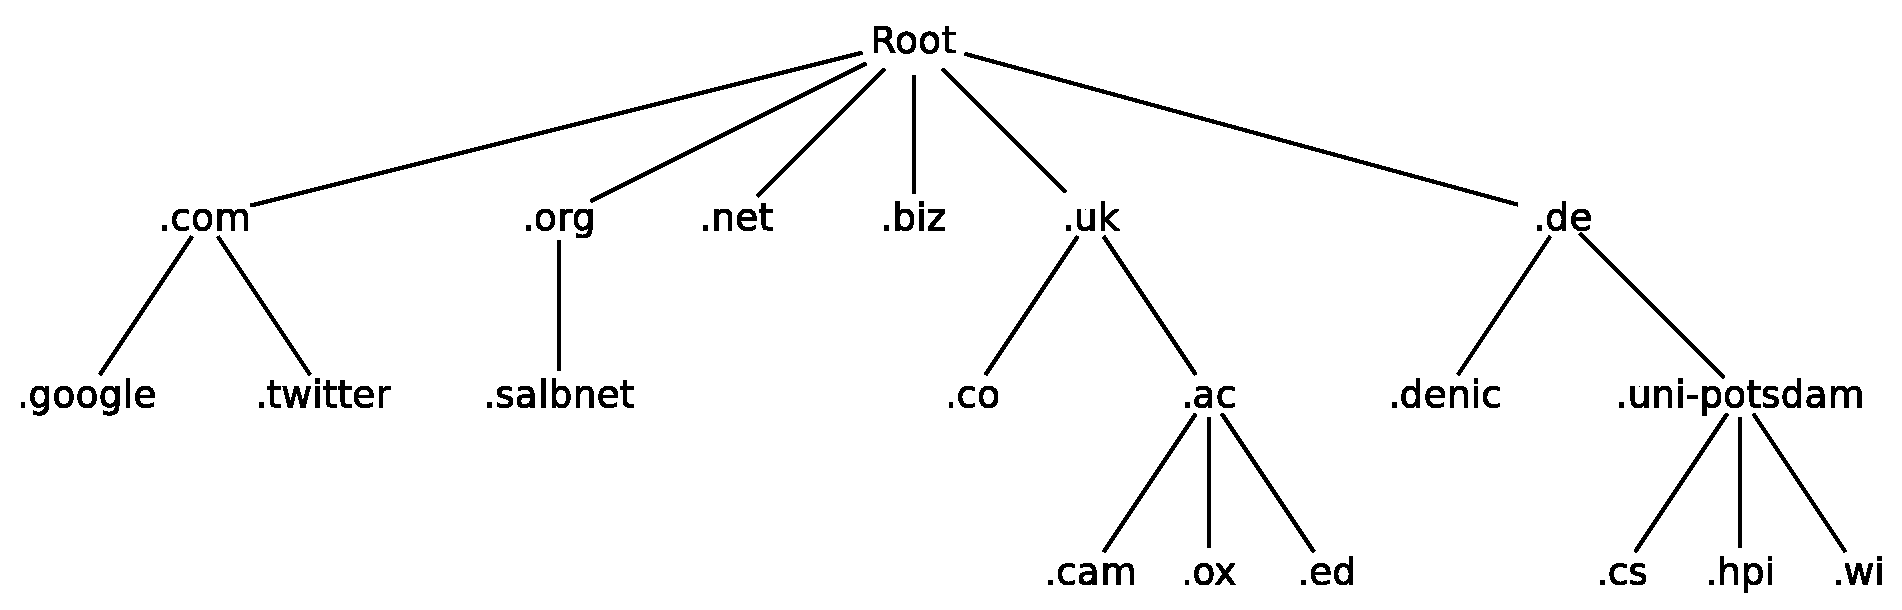
\includegraphics[width=\textwidth]{images/dns-tree-domains}
				\caption{Ausschnitt aus der DNS-Topologie} % TODO: schön machen
				\label{fig:dns-tree}
			\end{figure}

			Der Vorteil in der Speicherung der DNS-Informationen in einem Baum, ist dass jede Subdomain
			nur Informationen zu dem darunter liegenden Teilbaum speichern muss. Das heißt, die Subdomain
			\texttt{de} besitzt Informationen bezüglich den Subdomains \texttt{denic} und
			\texttt{uni-potsdam} aber keine Informationen bezüglich \texttt{com} oder \texttt{net}.
			Dadurch wird einer Seits die Menge an Informationen je Knoten gering gehalten und außerdem
			kann so die Verwaltung und Pflege der Information an verschieden Betreiber delegiert werden.

			Die Root-Domain wird von der Internet Corporation for Assigned Names and Numbers (ICANN)
			kontrolliert und auch die Vergabe der Top-Level-Domains (TLDs) ist an sie gebunden. Die ICANN
			ist eine Non-Profit-Organisation mit Sitz in den USA. Sie ist zwar für die Vergabe der TLDs
			verantwortlich, verwaltet und betrieben werden diese jedoch von verschieden Organisationen und
			Unternehmen. Es existieren aktuell 313 TLDs \cite{tlds}, welche sich hauptsächlich in drei
			Arten unterteilen lassen:

			\begin{itemize}
				\item länderspezifische \textit{country-code TLDs} (ccTLDs)
				\item allgemeine \textit{generic TLDs} (gTLDs):
				\begin{itemize}
					\item von ICANN verwaltete \textit{unsponsored TLDs} (uTLDs)
					\item von privaten Organisationen vorgeschlagene \textit{sponsored TLDs}
						(sTLDs)
				\end{itemize}
			\end{itemize}

			In der Abbildung \ref{fig:dns-tree} sind zum Beispiel die Domains \texttt{uk} und \texttt{de}
			ccTLDs, die Domains \texttt{com}, \texttt{org} und \texttt{net} sind uTLDs, und \texttt{mobi}
			ist eine sTLD. Unter den TLDs folgen die sogenannten Second-Level-Domains (SLDs), welche meist
			schon zu den eigentlichen Netzteilnehmern gehören oder noch eine weitere Einteilungsebene
			einführen. So gibt es zum Beispiel in der englischen \texttt{uk}-Domain noch die
			\texttt{co}-Domain für Firmen oder die \texttt{ac}-Domain für akademische Einrichtungen. Die
			\texttt{uni-potsdam}-Domain in der \texttt{de}-Domain wird allerdings bereits direkt von der
			Universität Potsdam verwaltet. Die Universität Potsdam unterteilt ihre eigene SLDs wiederum
			weiter in Subdomains, zum Beispiel für die einzelnen Institute (\texttt{cs} für das Institut
			für Informatik). Diese Domains können dann wiederum von den einzelnen Instituten verwaltet und
			weiter unterteilt werden.

			\lstinputlisting[float,caption={Ausschnitt eines Master-Files},label=lst:master]{listings/master-file}

			Dieser dezentrale Ansatz hat eine Reihe von Vorteilen. Als wichtigster Punkt ist die
			Verteilung der Last zu nennen, womit sowohl der Aufwand zur Wartung einer Domain, als auch zur
			Verteilung der Informationen gemeint ist. Zusätzlich ist es für die Betreiber einer Domain
			einfacher Änderungen einzupflegen. Da ein Betreiber alle Subdomains seiner eigenen Domain
			alleine verwalten kann spricht man bei der Verwaltung und Konfigurationen von \textit{Zonen}.
			Eine Zone umfasst alle Domains, welche von diesem DNS-Betreiber verwaltet werden. So gehören
			zum Beispiel alle Subdomains von \texttt{haiti.cs.uni-potsdam.de} zu einer Zone. Diese Zonen
			werden über sogenannte Master-Files \cite{rfc1035,liualb2006} verwaltet. Listing
			\ref{lst:master} zeigt einen Auszug aus einem Beispiel für ein Master-File. Der grundlegende
			Aufbau ist in der Form: Domain-Name (Vollständig mit abschließendem Punkt oder Subdomain),
			Klasse (IN für Internet), Typ (optionale weitere Parameter für spezielle Typen z.B. bei MX)
			und abschließend die gespeicherte Information. In Listing \ref{lst:master} sind in Zeile 1-2
			zwei \texttt{NS}-Einträge, diese geben die Nameserver einer Domain an. Zeile 4 ist ein Eintrag
			für einen Mailserver (\texttt{MX}), dieser erhält zusätzlich einen Präferenz-Wert (10),
			welcher bei mehreren Mailservern die Ordnung dieser definiert. Anschließend folgen in Zeile
			6-9 vier IPv4-Adressen (\texttt{A}) für verschiedene Subdomains. Und in Zeile 11 ist der Alias
			(\texttt{CNAME}) \textit{www} für die  \textit{twix}-Domain definiert. Diese Beispiel zeigt
			nur eine kleine Anzahl von möglichen Typen, deshalb sind in Tabelle \ref{tab:dns-types} die
			wichtigsten von ihnen aufgeführt.

			\begin{table}
				\centering
				\begin{tabular}{|c|l|}\hline
					Typ & Beschreibung \\\hline\hline
					A	& IPv4-Adresse\\
					AAAA	& IPv6-Adresse\\
					NS	& Nameserver\\
					MX	& Mailserver\\
					CNAME	& Kanonischer Name eines Alias\\
					SOA	& Start einen Zonenautorität\\
					PTR		& Zeiger von eine Adresse auf eine Domain\\\hline
				\end{tabular}
			\caption{Die wichtigsten Eintragstypen in einem DNS-Master-File \cite{rfc1035,rfc3596}}
			\label{tab:dns-types}
			\end{table}

			Diese Master-Files werden von DNS-Servern gelesen und verarbeitet. Es gibt verschiedene Arten
			von DNS-Server, welche bestimmen wie der DNS-Server auf Anfragen antwortet. Dabei
			unterscheidet man in iterative und rekursive Nameserver.

			\subsubsection*{Iterative Nameserver} % {{{

			Ein iterativer Nameserver kennt nur die Informationen aus seinem eigenen Master-File, also
			seiner eigenen Zone. Erhält ein iterativer Nameserver eine Anfrage außerhalb seiner Zone, kann
			er diese nicht beantworten und senden deshalb die Adressen der Server zurück, welche für die
			Root-Domain verantwortlich sind. Diese Adressen sind jedem DNS-Server bekannt. Das Ziel dieses
			Verhaltens ist es auf dem DNS-Server keine unnötige Last zu erzeugen und die Antwortzeit so
			gering wie möglich zu halten. Daraus lässt auch der Haupteinsatzort für solche Nameserver
			ableiten. Alle Server, welche die Root-Domain verwalten und die TLDs sind iterative
			Nameserver. Sie erhalten die meisten Anfragen und müssen diese schnell und effizient
			verarbeiten. Auch die meisten DNS-Server von Firmen, welche vom Internet erreichbar sind,
			werden ebenfalls iterative Nameserver sein.

			% subsubsection Iterative Nameserver }}}

			\subsubsection*{Rekursive Nameserver} % {{{

			Das Gegenteil zu iterativen sind rekursive Nameserver. Auch sie beantworten Anfragen bezüglich
			der eigenen Zone, wenn sie jedoch eine Anfrage außerhalb ihrer Zone erhalten fragen sie selber
			bei anderen Nameservern nach der Antwort. Das heißt der gefragte rekursive Nameserver
			unternimmt den Aufwand und ermittelt selber die Antwort auf die gestellte Frage und sende
			diese dann an den Fragenden zurück. Um dieses Vorgehen effizienter zu gestalten werden häufig
			Caches eingesetzt. In ihnen werden die ermittelten Informationen, welche außerhalb der eigenen
			Zone liegen, gespeichert. Dadurch können Anfragen schneller beantwortet werden, falls die
			Antwort bereits im Cache existiert, oder es kann schneller die Antwort gefunden werden, falls
			im Cache bereits Informationen zu Nameserver in der Nähe der Domain existieren. Das heißt,
			wenn die Domain \texttt{haiti.cs.uni-potsdam.de} angefragt wird und im Cache bereits die
			Adresse des \texttt{uni-potsdam.de}-Nameservers gespeichert ist, kann die Antwort schneller
			gefunden werden, als wenn der Nameserver sich von der Root-Domain durchfragen müsste.

			Rekursive Nameserver werden vor allem im privaten Netzwerken eingesetzt, wie zum Beispiel im
			Heimnetzwerk oder im firmeninternen Netzwerk, aber auch bei Internet Service Providern
			(ISPs). An diesen Punkten im Internet machen solche rekursiven Nameserver am meisten Sinn,
			dort treffen häufig die gleich oder zu mindestens ähnliche Anfragen ein. So kann man meist
			davon ausgehen das diese Nameserver immer die aktuelle Adresse von \texttt{google.com} und
			\texttt{wikipedia.org} etc. im Cache gespeichert haben. Und dieses Speichern von Informationen
			ist nicht nur vorteilhaft für die Nutzer, sondern verringert auch die Last auf den anderen
			DNS-Server im Internet. Ohne Nameserver mit Cache wäre die Last auf dem DNS-Netzwerk wohl um
			einiges höher. Allerdings gelten die Informationen eines DNS-Servers nicht unendlich lange,
			jede Antwort enthält eine maximale Lebensdauer der Information, danach ist sie nicht mehr
			gültig und sollte nicht weiterverwendet werden. Das heißt auch das sie aus dem Cache entfernt
			und neu abgefragt werden muss. Dies ist jedoch nötig, da sonst nie Änderung in einer Zone
			weiter propagiert würden.

			% subsubsection Rekursive Nameserver }}}

			\subsubsection*{Resolver} % {{{

				\begin{figure}
					\centering
					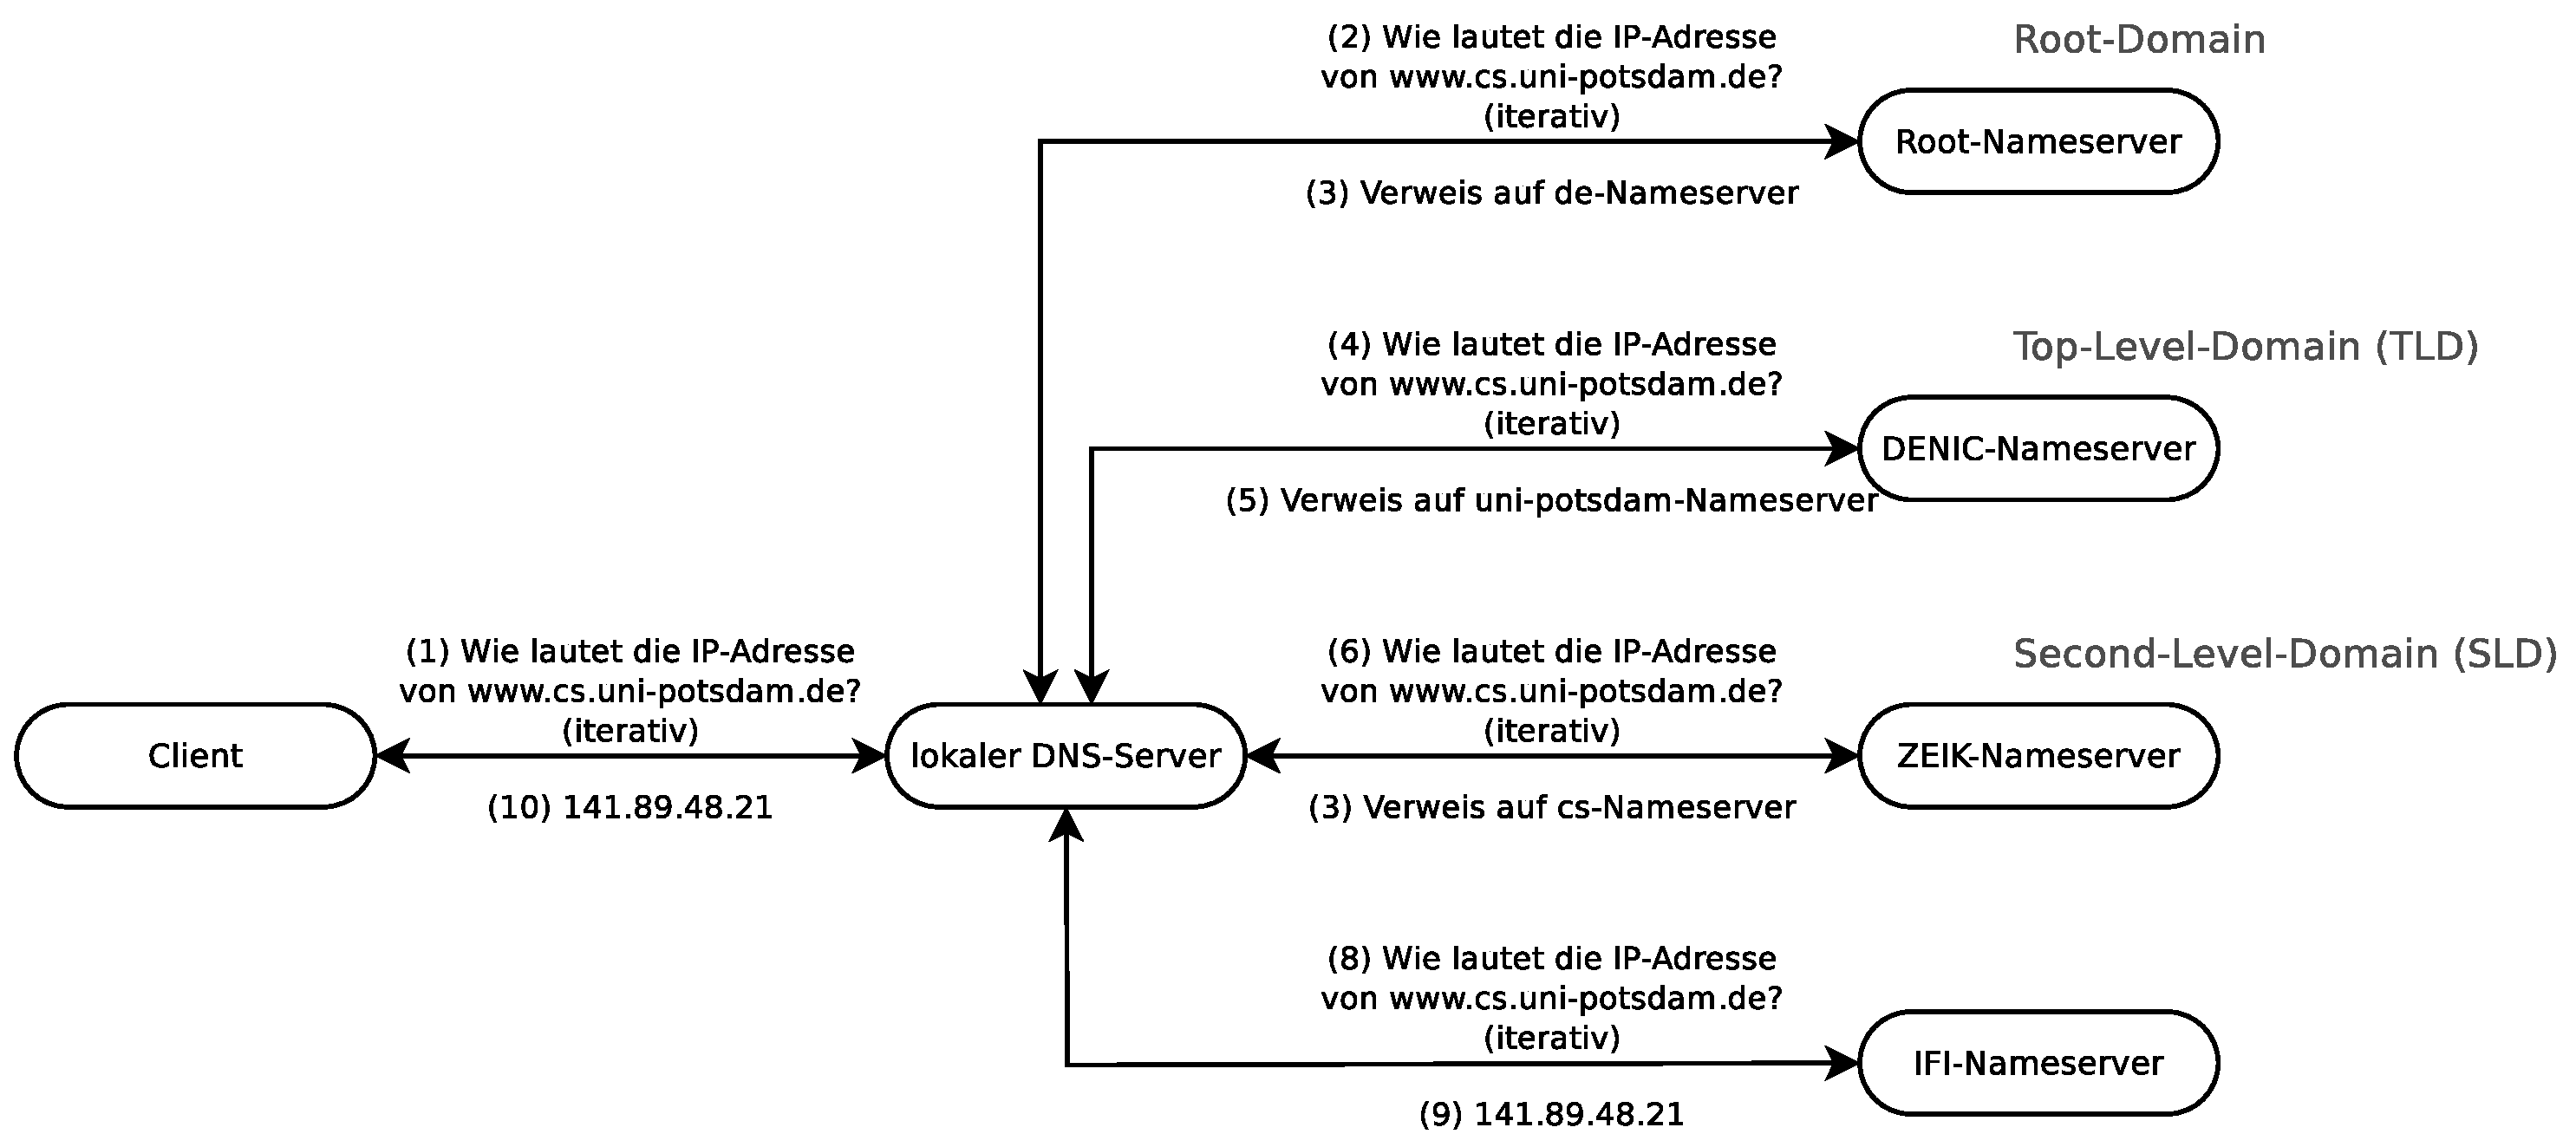
\includegraphics[width=\textwidth]{images/request}
					\caption{DNS-Anfragen für \texttt{www.cs.uni-potsdam.de}} % TODO: schön machen
					\label{fig:bsp-request}
				\end{figure}

				Damit eine Anwendung, wie zum Beispiel ein Webbrowser oder ein E-Mail-Client, Adressen
				auflösen kann, wird ein sogenannter Resolver benötigt. Seine Aufgabe ist es für die
				Anwendung einen Domain-Namen zu der entsprechenden IP-Adresse aufzulösen. Das heißt, wenn
				der Resolver von einer Anwendung die Anfrage nach der Adresse \texttt{www.cs.uni-potsdam.de}
				erhält, erzeugt der Resolver eine gültige DNS-Anfrage \cite{rfc1035} nach eben dieser
				Adresse und sendet diese an den im Betriebssystem konfigurierten primären DNS-Server. Dabei
				handelt es sich meist um einen rekursiven Nameserver, welcher dann selber einen Resolver
				nutzt um weitere Anfragen zu stellen, sofern er die Antwort nicht im Cache gespeichert hat.
				In Abbildung \ref{fig:bsp-request} ist der Ablauf der Beispiel-Anfrage dargestellt. Der
				Resolver des Clients sendet die Anfrage (1) an den lokalen DNS-Server. Dieser ist rekursiv
				und ermittelt deshalb nun die Antwort (Annahme: Der Cache des DNS-Servers enthält keine
				relevanten Informationen). Die Anfrage (2) wird deshalb an einen Root-Nameserver gestellt,
				da der lokale DNS keine anderen Informationen bezüglich der Domain besitzt. Der
				Root-Nameserver besitzt nur die Information, welcher Nameserver für die \texttt{de}-Domain
				verantwortlich ist und sendet diese Antwort (3) an den lokalen DNS-Server zurück. Dieser
				befragt (4) anschließend den \texttt{de}-Nameserver, welcher wiederum ein iterativer
				Nameserver ist und somit nur die \texttt{uni-potsdam}-Domain kennt (5). Die Anfragen an den
				\texttt{uni-potsdam}-Nameserver (6) liefert die Adresse des zuständigen Nameservers zurück
				(7). Dieser kann nun auf die letzte Anfrage (8) mit der gewünschten Adresse antworten (9).
				Welche dann vom lokalen DNS-Server an den Client zurückgeliefert wird (10). Alle
				Informationen, die in den Zwischenanfragen gesammelt wurden, werden im Cache des lokalen
				DNS-Servers gespeichert. Das heißt würde der Client nun erneut nach der Adresse
				\texttt{www.cs.uni-potsdam.de} fragen, könnte der lokale DNS-Server sofort antworten. Oder
				wenn die Anfrage diesmal \texttt{haiti.cs.uni-potsdam.de} wäre, würde der lokale DNS-Server
				sofort beim \texttt{cs.uni-potsdam.de}-Nameserver anfragen, da er dessen Adresse bereits
				kennt und weißt das dieser für die Domain zuständig ist.

			% subsubsection Resolver }}}

			\subsubsection*{DNS Security Extension} % {{{

				Mit der DNS Security Extension (DNSSEC) \cite{rfc4033,rfc4034,rfc4035,liualb2006} wurde ein
				neuer Standard eingeführt, welcher das DNS absichern soll. Es gibt verschiedene
				Angriffsszenarien auf das DNS \cite{lorenz2012}, wo durch Informationen verändert und somit
				ganze Domains übernommen werden können. Mit DNSSEC soll die Authentizität und
				Datenintegrität der Informationen gewährleistet werden und überprüfbar sein. Dazu werden
				kryptographische Verfahren eingesetzt. Die Einführung und Umstellung auf DNSSEC ist zu
				diesem Zeitpunkt noch nicht abgeschlossen, jedoch ergeben sich daraus interessante
				Überlegungen bezüglich der Last auf dem DNS-Netzwerk. Durch die kryptographische
				Abschicherung werden die DNS-Nachrichten größer und Resolver müssen kryptographische
				Methoden nutzen, was die eine höhere Rechenleistung beim Client voraussetzt. So bald das
				System vollständig eingeführt wurde, wird es interessant sein zu untersuchen, in welcher
				Form sich die Veränderung auf die Auslastung des DNS auswirkt.

			% subsubsection DNSsec }}}

			% subsection Aufbau }}}

			\subsection{DNS-Server Software} % {{{
			\label{sub:software}
			
				In diesem Abschnitt werden mehrere Softwaresysteme vorgestellt, welche zum Betrieb eines
				DNS-Server genutzt werden. Diese wurden aufgrund von zwei Studien aus den Jahren 2004 und
				2009 zur Verteilung von DNS-Server Software ausgewählt. Die erste Studie \cite{survey2004}
				wurde am 23. Mai 2004 abgeschlossen und untersuchte 37.836.997 SLDs unter den TLDs
				\texttt{com}, \texttt{net}, \texttt{org},	\texttt{info} und \texttt{biz}. Die zweite Studie
				\cite{survey2009} ist vom Oktober 2009, dabei wurden 3.308.662 SLDs unter den TLDs
				\texttt{com}, \texttt{net} und \texttt{org} untersucht. Es wurde jeweils versucht die
				eingesetze DNS-Server Software zu ermitteln. Dabei wurden die Systeme BIND, djbdns,
				Microsoft DNS und NSD als vier der häufigsten Systeme ermittelt (siehe Tabelle
				\ref{tab:verteilung}). Die genannten vier Systeme werden im folgenden vorgestellt.
				Zusätzlich wird auf den dnsmasq Server eingegangen, welcher eine sehr spezielle Form eines
				DNS-Servers darstellt.
				
				\begin{table}
					\centering
					\begin{tabular}{|c|c|c|}\hline
						DNS-Server & 2004 & 2009 \\\hline\hline
						BIND & \unit[70,11]{\%} & \unit[73,85]{\%} \\
						djbdns & \unit[15,57]{\%} & \unit[2,56]{\%} \\
						Microsoft DNS & \unit[6,24]{\%} & \unit[0,26]{\%}\\
						NSD & \unit[0,20]{\%} & \unit[0.03]{\%} \\\hline
					\end{tabular}
					\caption{Verteilung von DNS-Server Software nach \cite{survey2004, survey2009}}
					\label{tab:verteilung}
				\end{table}

				\subsubsection*{BIND} % {{{

				Die erste Version des Berkeley Internet Name Domain
				(BIND) \cite{bind} Server wurde am Anfang der achtziger Jahre
				an der University of California, Berkeley entwickelt und mit 4.3BSD erstmals
				veröffentlicht. Inzwischen wird BIND von dem Internet Systems Consortium (ISC)
				weiterentwickelt und gepflegt. BIND hat sich zu dem De-facto-Standard für DNS-Server
				entwickelt. Er wird auf 10 der 13 Root-Server eingesetzt und ist auch sonst bei TLDs
				weitverbreitet. Die erste Version des aktuellen BIND 9 Servers wurde 2000 veröffentlicht,
				ein Nachfolger wird seit 2 Jahren entwickelt um die aktuellsten Standards (z.B.  DNSsec) zu
				unterstützen.

				Für diese Arbeit wurde der BIND Server als DNS-Server gewählt, da er der weitverbreitetste ist und
				ebenfalls am Institut für Informatik eingesetzt wird. Dadurch konnten Testmessungen in einem
				realistischen Umfeld mit realen Server-Logs ausgeführt werden. 
				
				% subsubsection BIND }}}

				\subsubsection*{Name Server Daemon (NSD)} % {{{

				Der Name Server Daemon (NSD) \cite{nsd} wird von den
				NLnet Labs entwickelt und hat als Hauptziel die Vielfalt unter den Root-Servern zu erhöhen.
				Das soll dazu führen, dass nicht alle Root-Server durch einen Fehler im BIND Server
				angreifbar sind. Aktuell nutzen auch bereits 3 der 13 Root-Server den NSD als DNS-Server.
				Mit der Zielsetzung vor allem auf Root-Server und TLD-Server eingesetzt zu werden, erklären
				sich auch die meisten Charakteristiken des NSD. Er ist ausschließlich ein autoritativer
				DNS-Server, das heißt er beantwortet keine rekursiven Anfragen. Was seinen Einsatz als
				DNS-Server in einem lokalen Netzwerk ausschließt. Daher kann bei dem NSD auf unnötige
				Funktionen verzichtet werden und somit auf hohe Belastbarkeit optimiert werden. Die erste
				Version der aktuellen NSD 3 wurde 2006 veröffentlicht.
				
				% subsubsection Name Server Daemon (NSD) }}}

				\subsubsection*{Microsoft DNS} % {{{

				Der Microsoft DNS Server \cite{msdns} ist eine Implementation
				von Microsoft, welche mit den Windows Server Produkten ausgeliefert wird. Er kann sowohl als
				authoritativer und rekursiver Nameserver betrieben werden. Durch seinen Einsatz auf Windows
				Servern kommt er vor allem in lokalen und Firmen-Netzwerken vor. Ein besonderes Merkmal des
				Microsoft DNS Servers ist, dass es nicht nur möglich ist die DNS-Informationen aus einem
				Master-File zu erhalten sondern auch aus einem Active Directory.
				
				% subsubsection Microsoft DNS }}}

				\subsubsection*{djbdns} % {{{

				Das von Daniel J. Bernstein entwickelte Software-Paket
				djbdns \cite{djbdns} ist einer der verbreitetsten DNS-Server. Daniel
				J.  Bernstein ist ein Mathematiker, Programmierer und Kryptologe aus den USA. Er
				veröffentlichte djbdns im Jahr 2001 und setzte eine
				Belohung \cite{guarantee} von \$1000 aus, für den ersten der
				einen Fehler in djbdns findet. Die Besonderheit von djbdns liegt darin, dass es ein
				Software-Paket aus mehreren Programmen ist, welche immer einen speziellen Einsatzzweck
				erfüllen. Somit verringert sich die Code-Basis und die Komplexität der Programme. Die
				Hauptkomponenten sind \texttt{tinydns} ein authoritativer Nameserver und \texttt{dnscache}
				ein rekursiver Nameserver. Für andere Funktionen wie das Austauschen von kompletten
				Zone-Informationen oder Blacklisting existieren ebenfalls eigene Programme.
				
				% subsubsection Djbdns }}}

				\subsubsection*{dnsmasq} % {{{

				Das Programm dnsmasq \cite{dnsmasq} wurde
				ausschließlich für Heim-Netzwerke entwickelt. Es stellt DNS und DHCP Dienste für ein kleines
				Netzwerk zur Verfügung. Dabei ist die Idee, dass dnsmasq die Netzwerkknoten im Heimnetz über
				DNS verfügbar macht, indem es entweder die \texttt{/etc/hosts} oder DHCP Informationen
				nutzt. Dadurch müssen die lokalen Rechner keine eigene \texttt{hosts}-Datei pflegen.
				Zusätzlich bietet es einen einfachn Cache für DNS-Anfragen, was zu einer Beschleunigung im
				lokalen Netz führen kann. Somit ist dnsmasq kein üblicher DNS-Server und eignet sich auch
				nicht zum Verwalten von Domains, zeigt jedoch eine alternative resourcenschonende lokale
				Verwendung des DNS auf.
				
				% subsubsection Dnsmasq }}}

			% subsection DNS-Server Software }}}

			
		% section Domain Name System (DNS) }}}

		\section{Lastverteilung} % {{{
		\label{sec:lastverteilung}

		\begin{figure}
			\centering
			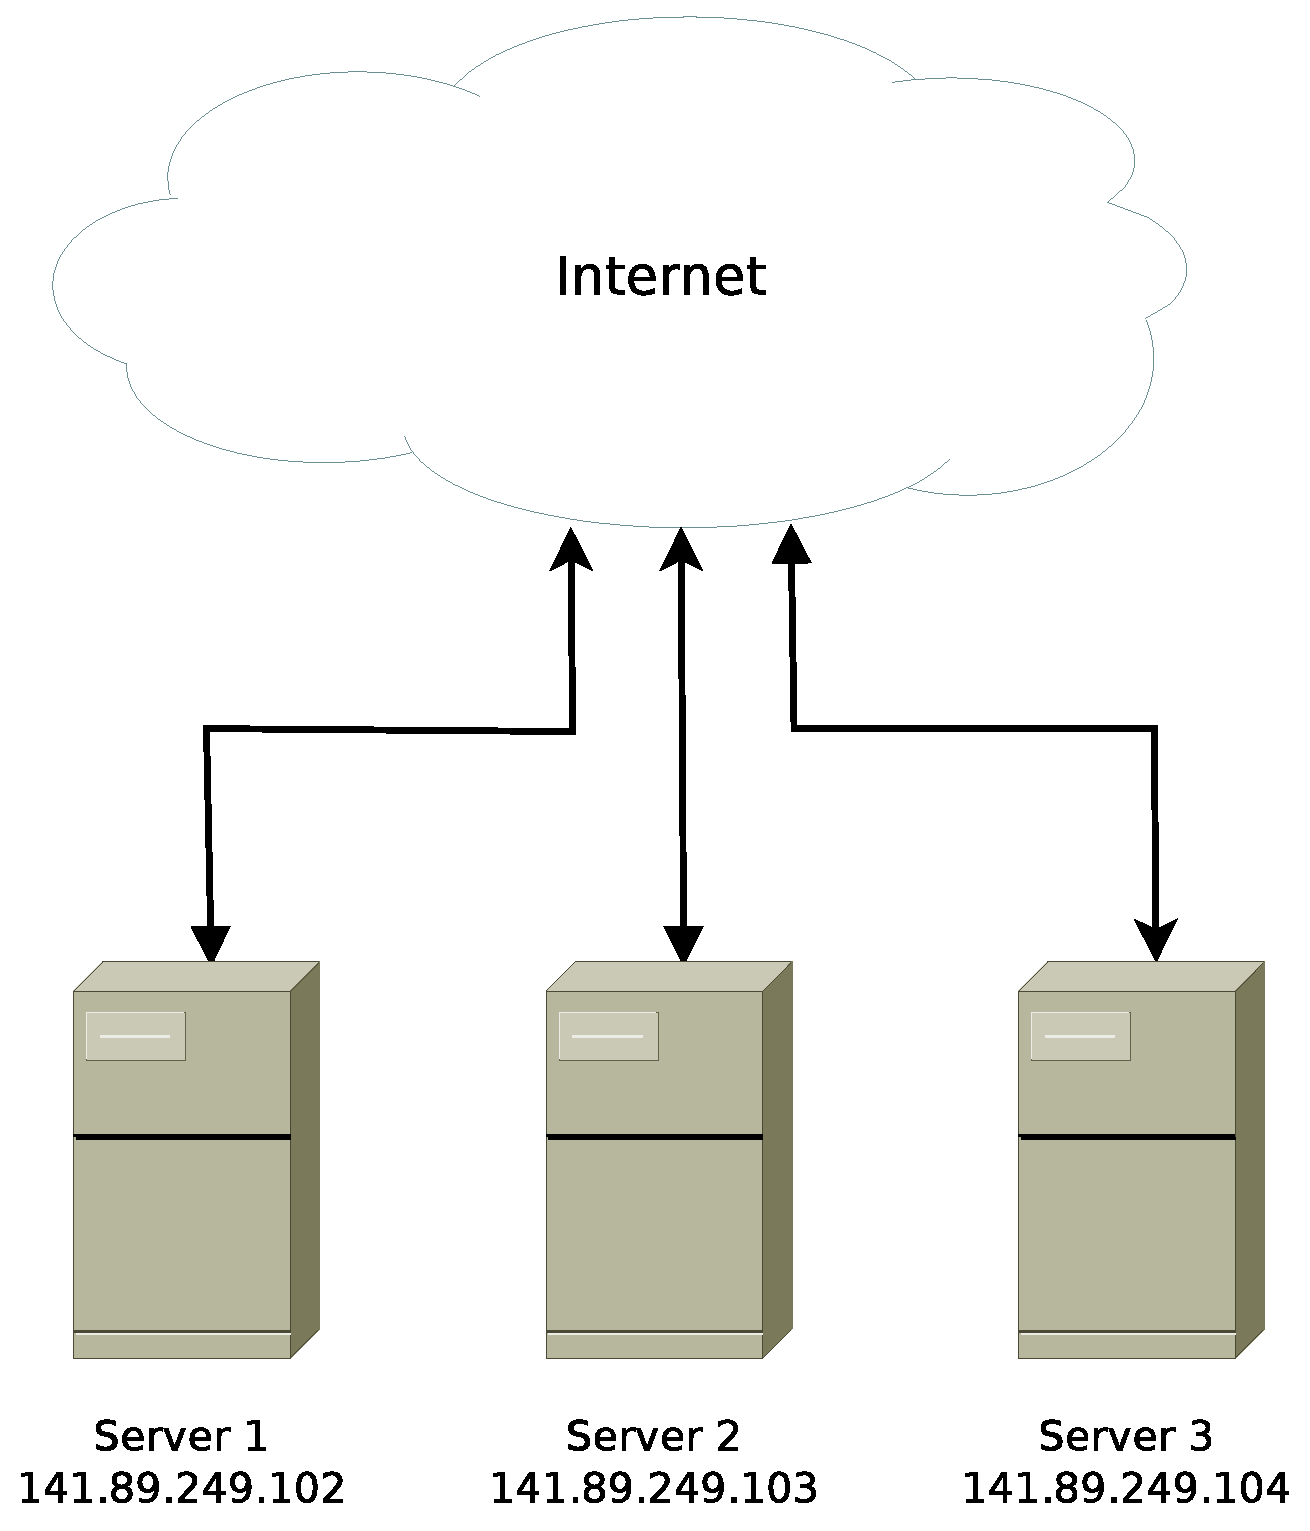
\includegraphics[width=6cm]{images/internet-server}
			\caption{Lastverteilung auf mehrer Server}
			\label{fig:lastverteilung}
		\end{figure}

		In diesem Abschnitt sollen Problemlösungen vorgestellt werden, welche dazu dienen die Last einer
		einzelnen Netzwerkressource zu verringern. Dies ist immer dann nötig und sinnvoll, wenn eine
		einzelne Ressource im Netzwerk einer so hohen Last ausgesetzt ist, dass sie diese nicht mehr
		allein abarbeiten kann. Zu hohe Last führt dazu, dass einzelne Anfragen an die Ressource nicht
		mehr beantwortet werden oder im ungünstigsten Fall ein Totalausfall droht. Ein häufiges Beispiel
		für hohe Lastsituationen sind Webserver, welche ab einer gewissen Anzahl an Anfragen pro Sekunde
		nicht mehr in der Lage sind alle Anfragen abzuarbeiten. Um die Überlastung einzelner Ressourcen
		zu verhindern gibt es zwei Möglichkeiten. Die erste Variante ist, die entsprechende Ressource
		durch eine leistungsfähigere Variante auszutauschen. Dies wird oft bei Datenbanken genutzt, wo
		der Server durch neue Hardware und bessere Ausstattung erweitert wird.  Für Datenbanken ist dies
		meist die einfachere Lösung, da es problematisch sein kann eine Datenbank zu verteilen und dabei
		die Daten konsistent zu halten. Die andere Variante ist eine Skalierung in die Breite, das heißt
		zum Beispiel einen weitere Server bereitzustellen. So kann der Dienst des Servers, wie in
		Abbildung \ref{fig:lastverteilung} zu sehen, von mehreren Servern dem Internet bereitgestellt
		werden. Dieses Vorgehen eignet sich oft bei Webservern, welche durch die Auslieferung von
		dynmaischen Inhalten (z.B. PHP-Seiten) ausgelastet sind. Das Skalieren in die Breite hat
		Vorteile gegenüber der ersten Variante und ist deshalb dieser vorzuziehen, sofern es die
		Anwendung zulässt.  Allein durch die Bereitstellung eines zusätzlichen Servers erhöht sich die
		Ausfallsicherheit und gleichzeitig auch die Wartbarkeit.  Durch diese Verteilung kann ein
		einzelner Server ausfallen oder überprüft werden, währende der andere Server die Anwendung
		weiterhin zur Verfügung stellt. Zudem ist die Erweiterbarkeit und weitere Skalierung sehr
		einfach, wenn einmal die Infrastruktur geschaffen wurde mehrere Server zu nutzen. Ein weiterer
		nicht zu vernachlässigender Punkt sind die Kosten. So ist die Anschaffung zweier identischer
		Systeme meist günstiger als ein einzelnes System, welches die gleiche Last verarbeiten kann.
		Hinzu kommt die Möglichkeit gezielt Ressourcen zu entfernen um Strom zu sparen. So könnten
		Server nur dann angeschaltet werden, wenn davon auszugehen ist, dass eine hohe Last bevorsteht.
		Ein Beispiel hierfür könnte eine Verkaufsplattform sein, die zusätzliche Ressourcen benötigt,
		wenn	besonders vor Feiertagen eine hohe Anzahl an Bestellungen eingeht.

		Im Folgenden werden verschiede Ansätze zur Verteilung von Last auf mehrere Systeme erläutert.
		Sie unterscheiden sich in der Umsetzung der Lastverteilung und bieten jeweils gewisse Vor- und
		Nachteile. Der Hauptanwendungsfall für diese Systeme ist die Verteilung von HTTP-Anfragen.
		Diese unterscheiden sich von DNS-Anfragen in mehreren Punkten, weshalb anschließend noch
		Besonderheiten und existierende Verfahren der Lastverteilung von DNS-Verkehr erklärt werden.

			\subsection*{Server-Lastverteilung} % {{{

			\begin{figure}
				\centering
				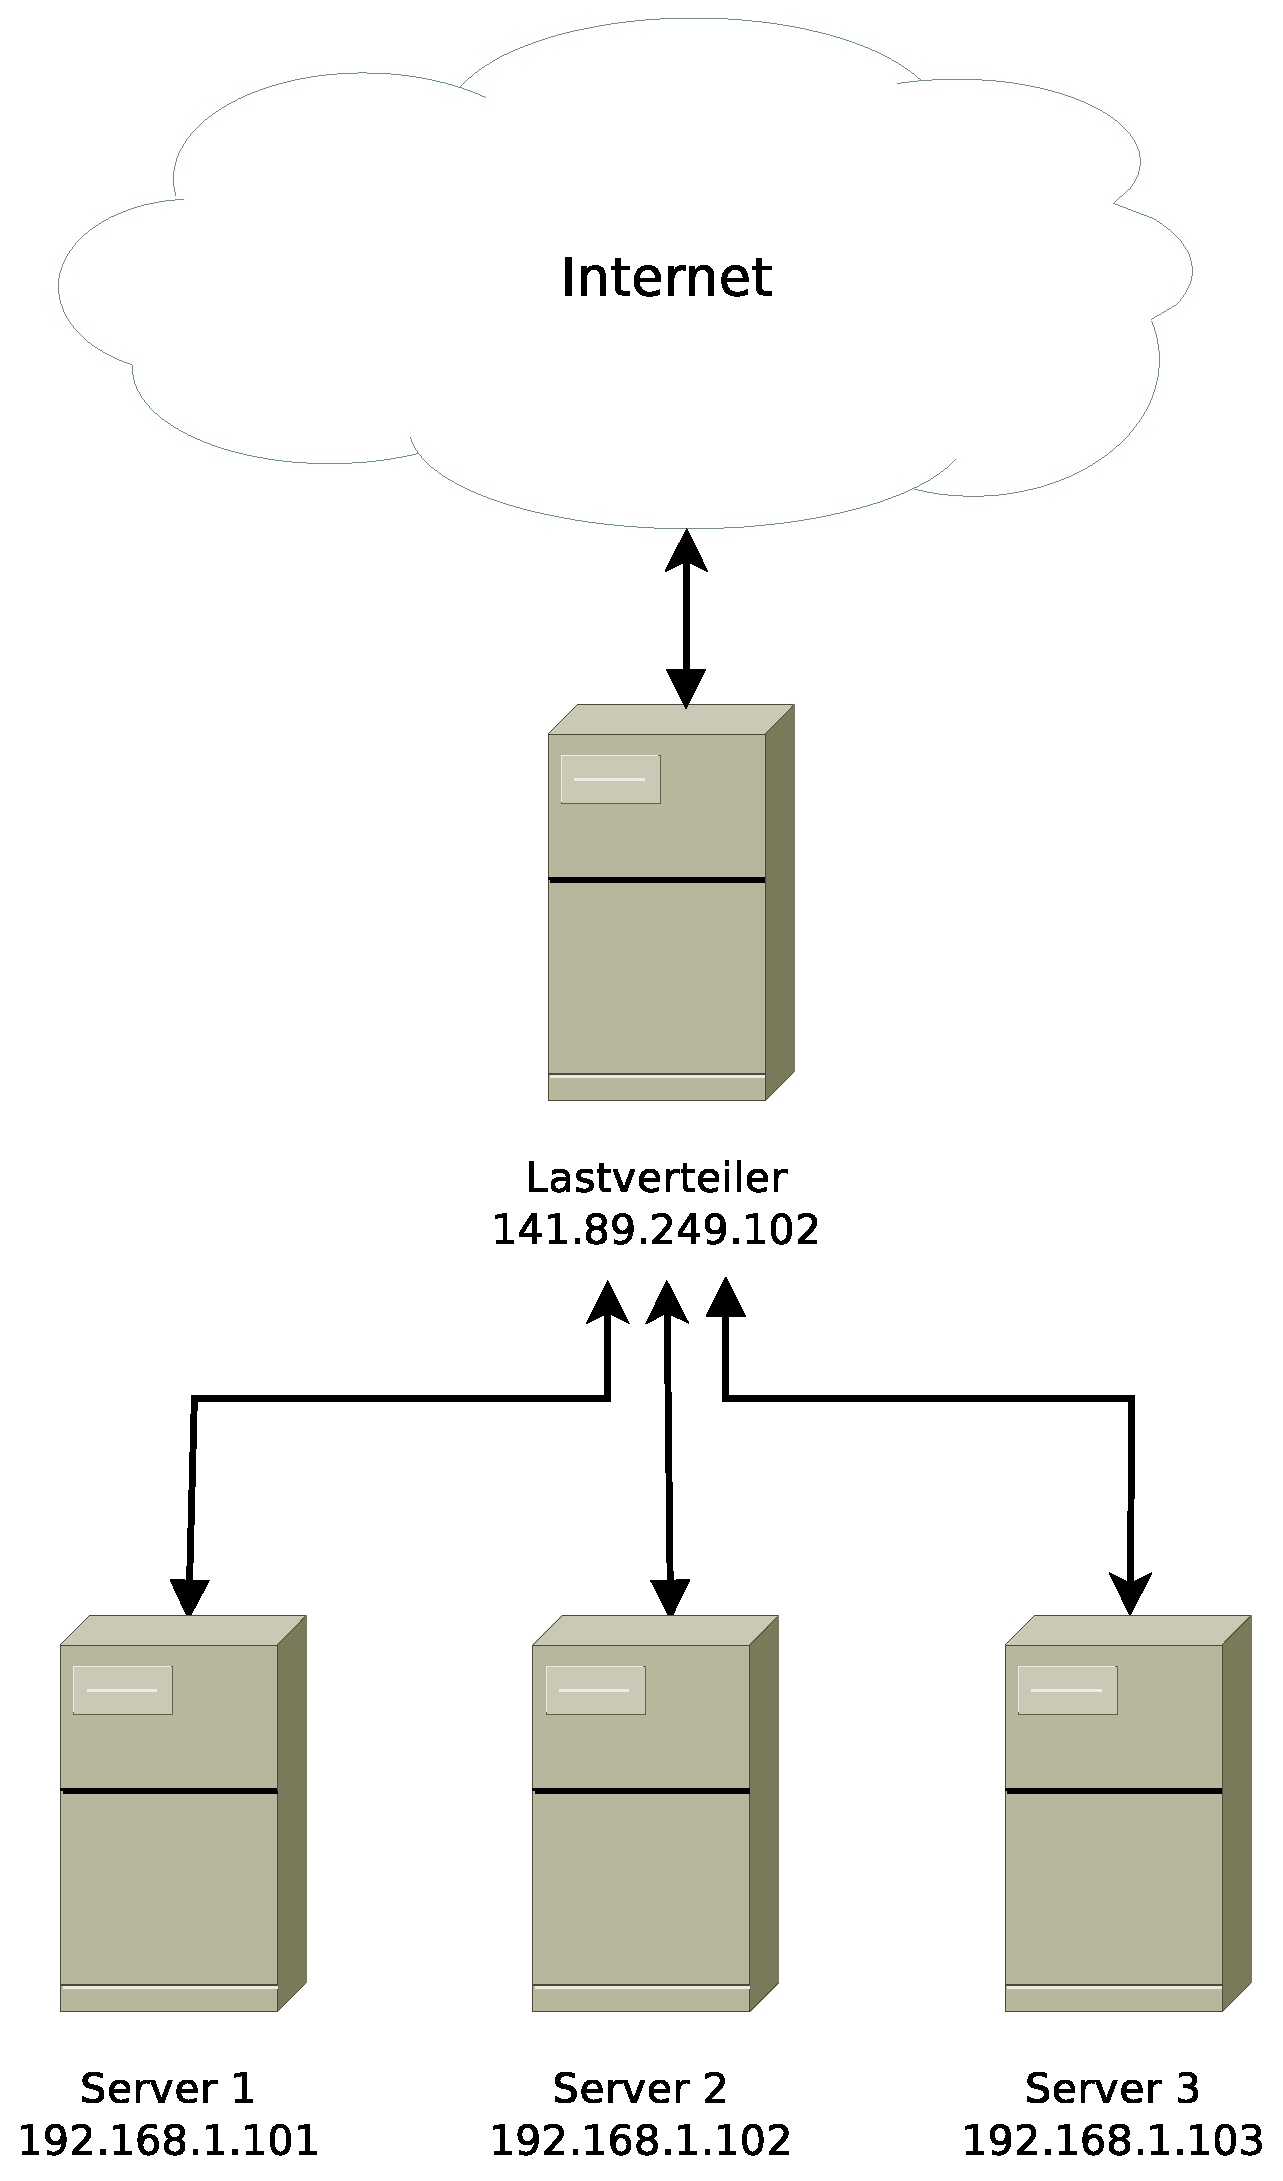
\includegraphics[width=6cm]{images/loadbalancer}
				\caption{Lastverteilung mit Hilfe eines Lastverteilers}
				\label{fig:loadbalancer}
			\end{figure}
			

			Bei dem Konzept der Server-Lastverteilung wird von der folgenden Situation ausgegangen.  Es
			existiert ein Cluster aus mehreren Servern, welche alle die selbe Anwendung (z.B. eine
			Website) zur Verfügung stellen. Diese sogenannten Backend-Server sind über einen
			Lastverteiler, einem weiteren Server, mit dem restlichen Netzwerk oder Internet verbunden
			(siehe Abbildung \ref{fig:loadbalancer}). Der Lastverteiler hat die folgenden Aufgaben
			\cite{bourke2001}:

			\begin{itemize}
				\item Entgegennehmen des kompletten Netzwerkverkehrs, welcher an die Anwendung gerichtet ist
					(z.B. HTTP-Anfragen an eine Website).
				\item Aufteilung des angenommenen Netzwerkverkehrs und Verteilung auf die Backend-Server.
				\item Beobachtung der Last der Backend-Server und entsprechenden Anpassung der
					Lastverteilung.
			\end{itemize}

			Diese Anforderungen können durch unterschiedliche Systeme realisiert werden. Es kann hierbei
			unterschieden werden ob ein Lastverteiler im Kernelspace oder Userspace des Betreibssystems
			implementiert ist. Ansätze für Userspace-basierte Lastverteiler sind zum Beispiel das Programm
			perlbal \cite{perlbal} oder das Apache-Modul mod\_proxy\_balancer \cite{modproxy}.  Eine
			Implementierung im Userspace hat den Vorteil, dass der Lastverteiler unabhängig von konkreten
			Betriebssystemen und Kernel-Versionen ist. Außerdem benötigt dieser keine \texttt{root}-Rechte
			um konfiguriert und gestartet zu werden. Da es sich um Anwendungen im Userspace handelt,
			findet hier die Lastverteilung auf einer höheren OSI-Schicht \cite{tanenbaum1988} statt.
			Dadurch stehen dem Lastverteiler anwendungsspezifischere Informationen zu einer Anfrage
			bereit. Dies kann zum Beispiel dazu genutzt werden, die Abfrage nach deren Inhalt zu filtern
			und so ein kontextsensitives Verteilen zu ermöglichen.  Ein Nachteil, welcher vor allem bei
			hohem Netzwerkverkehr zum Tragen kommt, ist der nötige Kontextwechsel damit der Lastverteiler
			im Userspace die Netzwerk-Pakete auswerten kann. Dazu muss das Netzwerk-Paket in den Userspace
			und zum Weiterversenden wiederum in den Kernelspace kopiert werden. Hierzu ist jeweils ein
			Kontextwechsel nötig, welcher bei hohem Netzwerkverkehr zu Leistungseinbußen führen kann
			\cite{boehme2006}.  Im Vergleich zu diesen Ansätzen im Userspace gibt es im Kernelspace den
			Linux Virtual Server (LVS) \cite{lvs,zhang2000} für Linux und den Paketfilter
			pf \cite{pf} für OpenBSD als bekannteste Beispiele.
			Indem die Pakete bereits im Kernelspace verarbeitet werden, findet kein Kontextwechsel statt
			und die Verarbeitung kann schneller erfolgen. Allerdings findet die Verarbeitung auf einer der
			unteren Schichten des OSI-Modells statt, was dazu führt das keine anwendungsspezifischen
			Informationen vorliegen. Jedoch bieten dieser Ansatz eben genau dies auch als Vorteil, denn so
			kann eine Lastverteilung unabhängig von Anwendungen statt finden.  Das heißt ein
			Lastverteiler, wie der LVS, kann so konfiguriert werden, dass er gleichzeitig
			unterschiedlichen Netzwerkverkehr (z.B. unterschiedliche Transportprotokolle oder Portnummern)
			separat verteilt. Dies ist mit einer anwendungsbasierten Lösung nicht ohne erheblichen Aufwand
			realisierbar.

			Unabhängig von der gewählten Software-Lösung ist der gewählte Algorithmus zur Lastverteilung
			ein entscheidendes Kriterium. Es existieren mehrere Algorithmen für dieses Problem
			\cite{zinke2007}, wobei es von der gewählten Software abhängt, welche zur Verfügung stehen.
			Die zwei bekanntesten Verfahren sind das Round-Robin-Verfahren und das
			Least-Connection-Verfahren. Beim Round-Robin-Algorithmus wählt der Lastverteiler, aus einer
			Liste von Servern, den nächsten aus. Dies geschieht zyklisch, was dazu führt, dass die
			Reihenfolge der Server immer gleich bleibt. Dies ist ein sehr einfacher Algorithmus der aber bei
			homogenen Clustern und homogenen Anfragen ausreicht um Last sinnvoll zu verteilen. Handelt es
			sich nicht um ein homogenes Cluster, so kann durch eine gewichtete Variante des Algorithmus
			die Last entsprechend der Leistung der Server verteilt werden. Sind jedoch die Anfragen an das
			Cluster nicht homogen, das heißt jede Anfrage erzeugt eine unterschiedliche Last bei den
			Backend-Servern, kann dies nicht durch den Round-Robin-Algorithmus ausgeglichen werden. Der
			zweite bekante Algorithmus ist Least-Connection. Dieser Algorithmus beachtet bei der
			Verteilung die aktuelle Anzahl an Verbindungen zu den Backend-Servern, das heißt wenn ein
			Server schneller seine Anfragen abarbeitet als ein anderer, erhält dieser Server früher wieder
			Anfragen. Auch von diesem Algorithmus gibt es eine gewichtete Variante, welche die bereits
			dynamisch getroffene Entscheidung noch einmal verbessern soll. Daher ist anzunehmen, dass
			Least-Connection bessere Ergebnisse auf heterogenen Clustern als Round-Robin erzielt und auch
			nicht homogene Anfragen begrenzt abfängt.

			% subsection Server Lastverteilung }}}

			\subsection*{DNS-basierte Lastverteilung} % {{{

			\begin{figure}
				\centering
				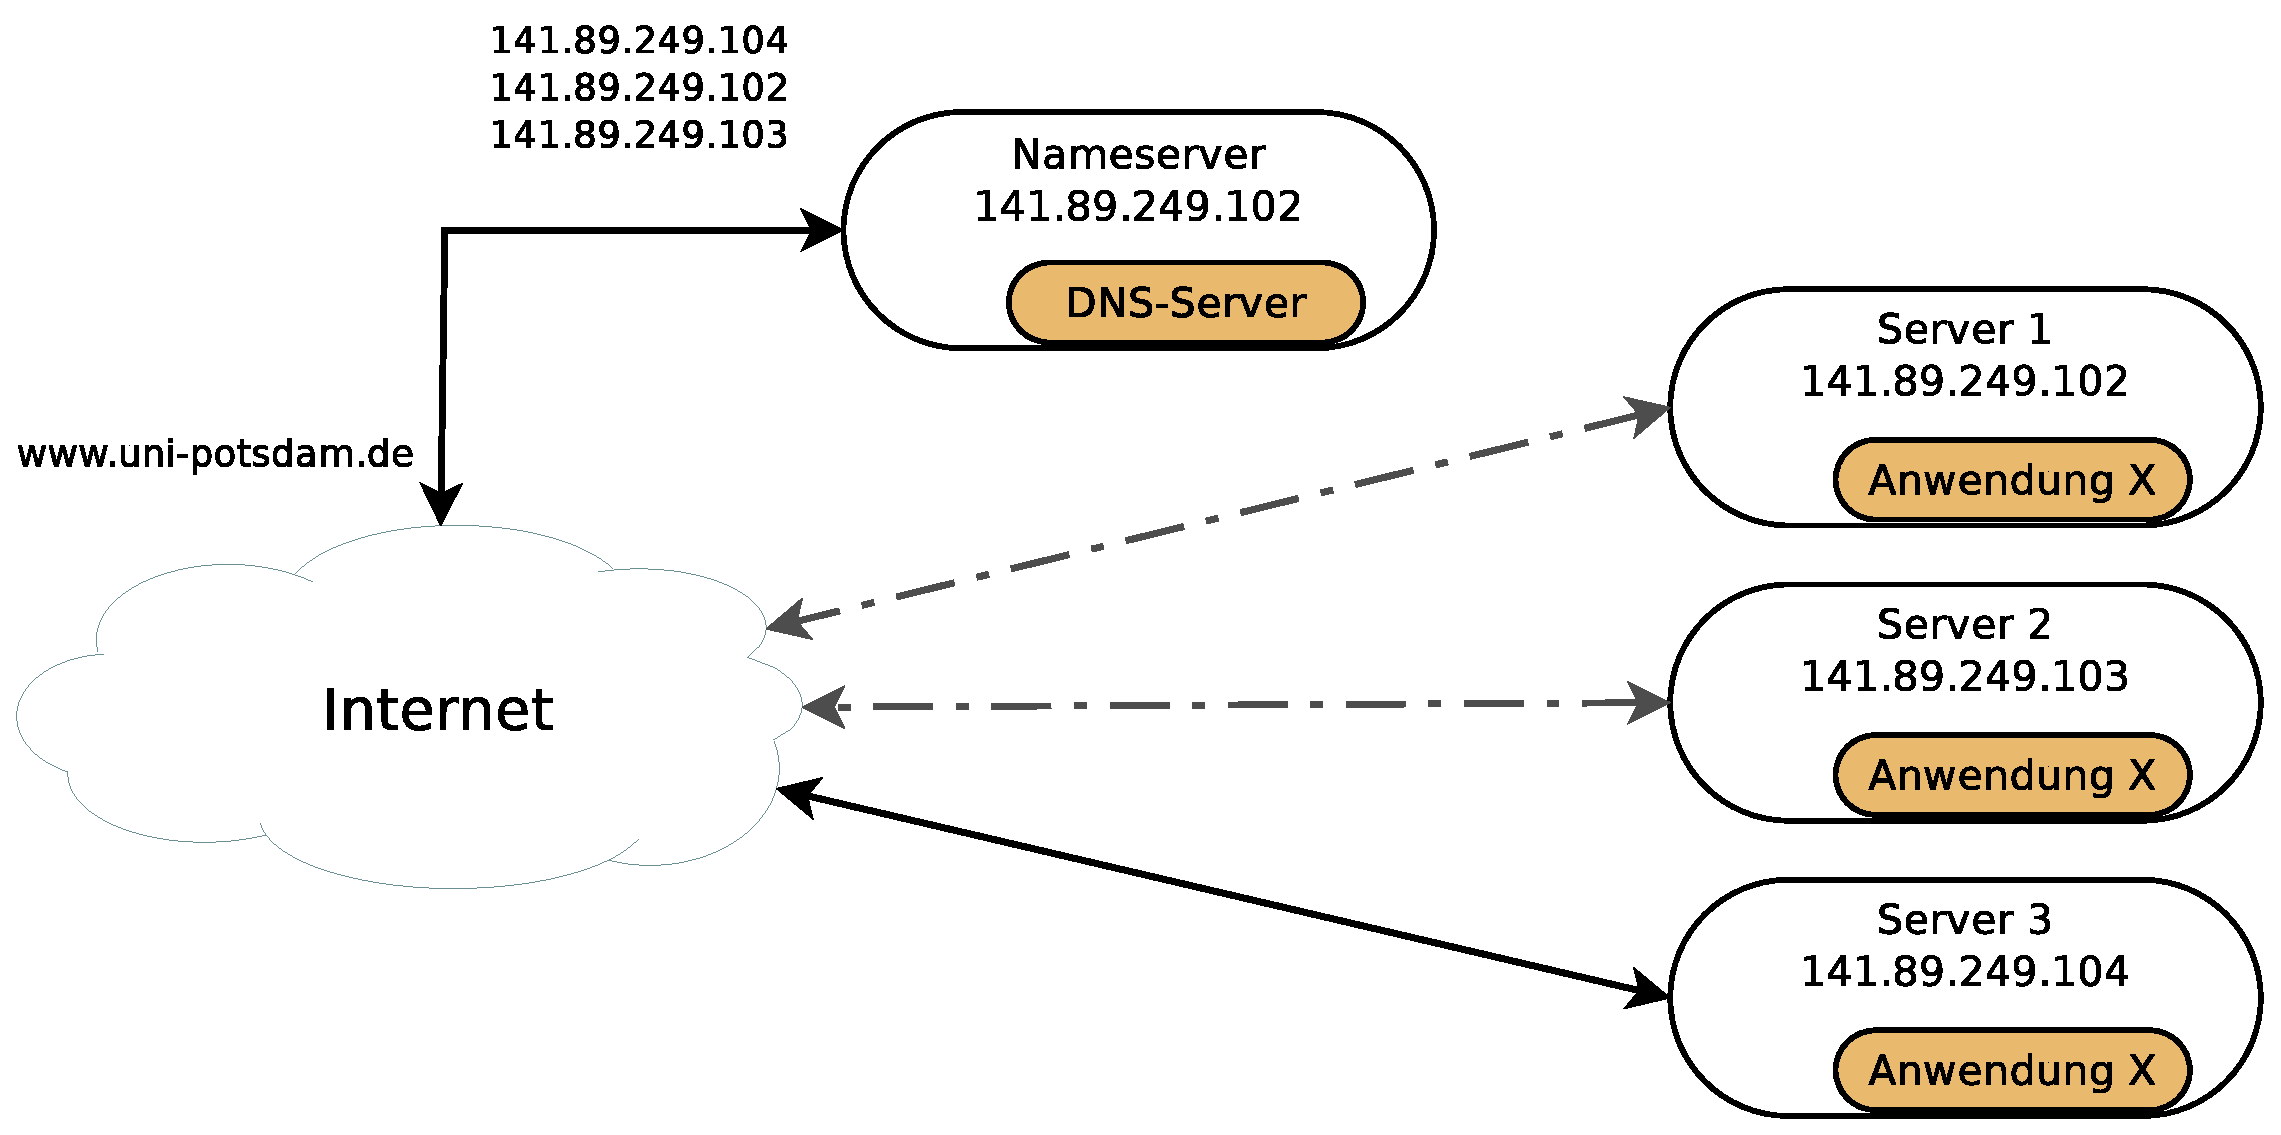
\includegraphics[width=10cm]{images/dns-loadbalancer}
				\caption{Lastverteilung mit Hilfe von DNS}
				\label{fig:lastverteilung-dns}
			\end{figure}

			Existiert kein Cluster oder es soll auf einen zusätzlichen Server verzichtet werden, bietet
			sich eine DNS-basierte Lastverteilung an. Diese nutzt die Möglichkeit, dass einem DNS-Eintrag
			für eine Domain mehrere IP-Adressen zugeordnet werden können \cite{rfc1034}. Ein möglicher
			Verbindungsablauf ist in Abbildung \ref{fig:lastverteilung-dns} dargestellt, dabei wird als
			erstes der DNS-Server befragt, welcher dann eine Liste alle möglichen Adressen liefert . Dabei
			existiert keine Ordnung dieser Einträge und der DNS-Server entscheidet, in welcher Reihenfolge
			er die IP-Adressen zurückliefert. Oft wird dazu ein Round-Robin-Algorithmus genutzt und somit
			eine gewissen Lastverteilung erreicht. Dieses Verfahren hat jedoch einige Nachteile. So führt
			das Caching von lokalen Nameservern dazu, dass alle Anfragen zu der Adresse im Cache geleitet
			werden. Weiterhin hat der DNS-Server keine Informationen über die Last der Server oder ob
			diese überhaupt im Betrieb sind. Dadurch wird ein Server der ausgefallen ist trotzdem immer
			wieder als Antwort zurückgeliefert. Auch ist es nicht möglich Gewichte für die Verteilung der
			Last auf den Server anzugeben, weshalb eine Heterogenität der Server nicht ausgeglichen werden
			kann. Dieses Problem sollte durch den Ressource Record Typen \texttt{SRV} \cite{rfc2782}
			behoben werden. Ein Beispiel eines \texttt{SRV}-Eintrags für einen Webserver ist in Tabelle
			\ref{tab:srv} zu sehen. Durch den Domain-Namen wird definiert, dass dieser Eintrag nur für
			HTTP-Anfragen über TCP an die Domain \texttt{bsp.de} gilt. In dem Beispiel wird anschließend
			den Domains \texttt{www.bsp.de} und \texttt{www2.bsp.de} eine Priorität von 0 und
			\texttt{backup.bsp.de} von 1 zugeordnet. Dabei muss von einem Client der Server mit der
			kleinsten Priorität gewählt werden, sofern dieser erreichbar ist. Gibt es mehrere Server mit
			der selben Priorität (wie im Beispiel \texttt{www.bsp.de} und \texttt{www2.bsp.de}), sollte
			die Wahl eines Server mit einem höheren Gewicht wahrscheinlicher sein. Zusätzlich wird noch
			der Port für das Ziel angegeben. Diese Verfahren führt zwei Gewichtungen ein, welche auf der
			Client-Seite ausgewertet werden. Allerdings ist dies das größte Problem. Denn die
			Unterstützung auf der Clientseite für \texttt{SRV}-Einträge ist gering. Außerdem bleibt das
			Problem bestehen, das der DNS-Server nicht die Last und Funktionstüchtigkeit der Server kennt.
			Jedoch gibt es dem Client einen Anhaltspunkt, welchen Server er als nächstes kontaktieren
			sollte, sofern ein Server nicht erreichbar ist.

			\begin{table}
				\centering
				\begin{tabular}{|ccccccl|}\hline
				 Domain & Klasse & RR & Priorität & Gewicht & Port & Ziel \\\hline\hline
					\_http.\_tcp.bsp.de. & IN & SRV & 0 & 2 & 80 & www.bsp.de. \\	
					& IN & SRV & 0 & 1 & 80 & www2.bsp.de. \\	
					& IN & SRV & 1 & 0 & 80 & backup.bsp.de. \\\hline
				\end{tabular}
				\caption{Beispiel für einen \texttt{SRV}-Eintrag für einen Webserver}
				\label{tab:srv}
			\end{table}

			Auch Kombinationen der Server-Lastverteilung und DNS-Lastverteilung sind möglich. Dabei wird ein
			DNS-Server um Lastverteilungsfunktionen erweitert. So beschreibt \cite{chyuyi2003} ein
			Verfahren, bei dem der DNS-Lastverteiler die Zeit überwacht, welche jeder Backend-Server für
			die Abfrage einer Antwort benötigt. Dadurch kann die DNS-Antwort entsprechend der
			Lastsitutation angepasst werden. Ein ähnlichen Ansatz beschreiben \cite{mookim2005}, dabei
			werden Backend-Server die überlastet sind aus der Round-Robin-Liste des DNS-Servers entfernt
			und dynamisch wieder hinzugefügt, sobald sie die Überlastsitutation überwunden haben. Bei dem
			allgemeinen Prinzip des Globalen Server-Lastverteilung \cite{bourke2001} kann der DNS-Server
			zum Beispiel anhand der geographischen Lage einen Server auswählen.

			% subsection DNS-basierte Lastverteilung }}}
			
			\subsection*{Lastverteilung von DNS-Verkehr} % {{{

			% TODO: das mit den Sessions überlegen

			Die Verteilung von DNS-Anfragen unterschiedet sich in mehreren Punkten von HTTP-Anfragen. So
			ist das genutzte Transport-Protokoll UDP statt TCP und die Nachrichten dürfen nicht größer als
			512 Byte sein \cite{rfc1035}. Weiterhin existieren beim DNS keine Client-Sessions wie bei
			HTTP-Anwendungen, wo ein Client während einer Session immer mit dem selben Server
			kommunizieren muss. Die Lastverteilung von DNS-Anfragen tritt jedoch wesentlich seltener auf
			als bei HTTP-Anfragen. Firmen und Organisationen haben selten einen so hohe Anzahl an
			DNS-Anfragen, dass sie eine Lastverteilung benötigen. Dies schließt nicht aus, dass mehrere
			DNS-Server existieren, welche aber oft nur als Schutz gegen Ausfällen und anderen Störungen
			dienen.  In lokalen Netzwerken und kleinere Firmen reicht es daher Lastverteilung mit Hilfe
			von DNS-Einträgen durchzuführen. Bei größeren Firmen, die eine höhere Anzahl an DNS-Anfragen
			zu bewältigen haben ist der Einsatz eines DNS-Clusters und Server-Lastverteilers sinnvoll. Die
			größte Last liegt bei den Betreiber von TLDs und den Root-Servern. Für diese Anwendungsfälle
			sind DNS-Cluster nötig. Zusätzlich kommt Anycast \cite{rfc4786, sapate2005} zum Einsatz. Dabei
			werden mehrere DNS Server mit der selben Anycast-IP-Adresse mit dem Internet verbunden. Sendet
			nun ein Client eine Anfrage an diese Anycast-Adresse antwortet der Server, der als erster die
			Frage erhält. Die Idee dahinter ist, dass durch den DNS-Server, der die kürzeste Route zum
			Fragesteller hat, die beste Antwort gegeben werden kann. Vor allem bei den Root-Servern ist
			dies sinnvoll. Es existieren insgesamt 13 Root-Server
			(A-M) \cite{rootserver}. Von ihnen nutzen 9 (A, C, F, G, I, J, K, L und M)
			Anycast-Adressen. Die anderen 4 Root-Server haben nur lokale Standorte in den USA. 
				
			% subsection Lastverteilung von DNS-Verkehr }}}

		% section Lastverteilung }}}

		\section{Fazit} % {{{
		\label{sec:grundlagen-fazit}
		
		% section Fazit }}}

  % chapter Grundlagen }}}

	\chapter{Verwandte Arbeiten} % {{{
	\label{cha:arbeiten}

	% TODO: DNS Measurements at a Root Server
	% TODO: DNS Cluster
	% TODO: DNS Root/gTLD Performance Measurement
	% TODO: Measurement of DNS Traffic Caused by DDoS Attacks
	% TODO: Measuring Availability in the Domain Name System
	% TODO: Two Days in the Life of the DNS Anycast Root Servers

	% chapter Verwandte Arbeiten }}}

	\chapter{salbnet} % {{{
	\label{cha:salbnet}

		Dieses Kapitel beschreibt salbnet \cite{salbnet}, einen Credit-basierten
		Lastverteilungsansatz.  Es basiert auf Arbeiten zur selbst-adaptiven Lastverteilung von
		TCP-Verkehr vor allem in InfiniBand-Netzwerken \cite{zinke2007, scsczile2008,
		schneidenbach2009}. Die Besonderheit an diesem Lastverteilungsverfahren ist, dass es sowohl eine
		Komponente auf dem Lastverteiler als auch auf den Backend-Servern gibt. Dabei werden auf den
		Backend-Servern Credits bestimmt, welche die Verfügbarkeit des Servers wiederspiegeln sollen,
		und an den Lastverteiler übermittelt werden. Der Lastverteiler wählt dann anhand der gemeldeten
		Credits die Backend-Server aus. Dieser Aufbau von salbnet ist in Abbildung \ref{fig:salbnet} zu
		sehen, wobei die Komponenten von salbnet blau hervorgehoben sind. Sie sollen im Folgenden kurz
		vorgestellt werden.

		\begin{figure}
			\centering
			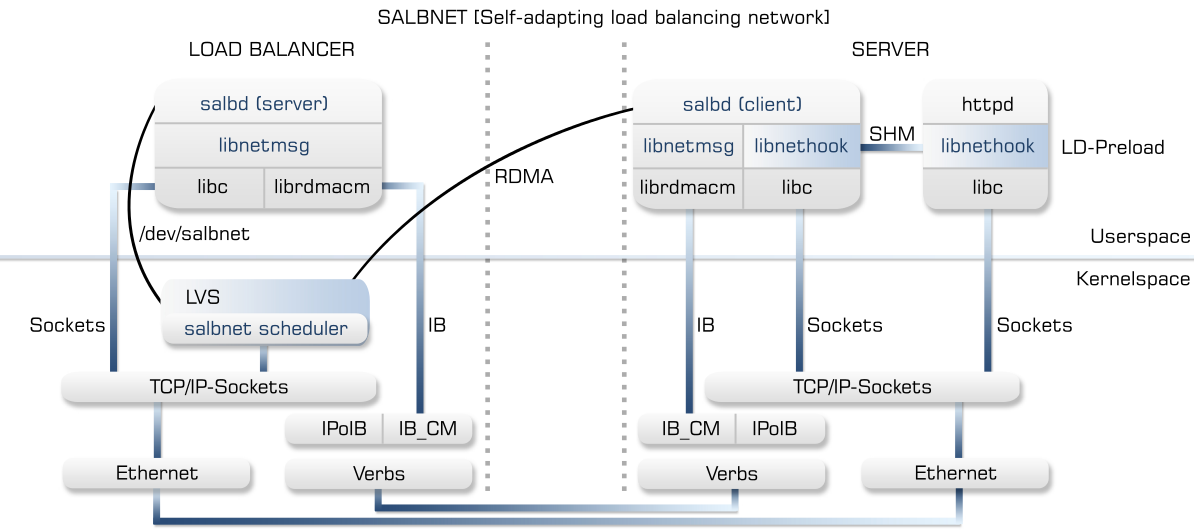
\includegraphics[width=\textwidth]{images/salbnet.png}
			\caption{Aufbau von salbnet (übernommen aus \cite{zinke2012})}
			\label{fig:salbnet}
		\end{figure}

		\subsection*{libnetmsg} % {{{

			Die libnetmsg \cite{rabweg2009} ist eine leichtgewichtige Kommunikations-Bibliothek die zur
			Übertragung sowohl UDP und TCP als auch InfiniBand unterstützt. Außerdem kann bei InfiniBand
			die Remote Direct Memory Access (RDMA) Eigenschaft genutzt werden. In salbnet wird die
			Bibliothek genutzt um die Credits von den Backend-Server an den Lastverteiler zu melden. Wird
			InfiniBand genutzt können die neuen Credits direkt in den Kernelspeicher des Lastverteilers
			geschrieben werden. Dieses Vorgehen ist in Abbildung \ref{fig:salbnet} dargestellt.

		% subsection libnetmsg }}}
		
		\subsection*{libnethook} % {{{

			Die dynamische Bibliothek libnethook wird genutzt um Funktionsaufrufe, von zu überwachenden
			Anwendungen abzufangen. So kann ermittelt werden wie oft eine Funktion aufgerufen wird und was
			von ihr zurück gegeben wird. Im Fall von salbnet, wird der \texttt{accept}-Funktionsaufruf vom
			Apache Webserver (httpd) \cite{httpd} abgefangen und analysiert. In
			Abbildung \ref{fig:salbnet} ist angedeutet, dass libnethook zwischen dem httpd und der libc
			aggiert. Allgemein kann das auch für alle anderen TCP-Anwendungen genutzt werden. Im TCP-Fall
			wird nur die Anzahl der Funktionsaufrufe genutzt um eine Neuberechnung der Credits auszulösen.

		% subsection libnethook }}}


		\subsection*{salbd} % {{{

			Die Hauptkomponente von salbnet ist salbd, welches sowohl auf dem Backend-Server als auch auf
			dem Lastverteiler zum Einsatz kommt. Auf dem Lastverteiler stellt salbd einmal ein Kernelmodul
			bereit, welches den salbnet scheduler für LVS implementiert. Dieser wählt Round-Robin den
			nächsten Backend-Server aus allen Servern, welche noch Credits größer 0 besitzen. Außerdem
			wird salbd genutzt um die Credits von den Backend-Servern zu empfangen und bei Übertragungen
			ohne RDMA auch um die Credits in den Kernelspace zum salbnet Scheduler zu übermitteln.  Im
			Backend ist salbd zur Bestimmung der Credits anhand der aktuellen Last der Webserver
			verantwortlich. Dazu werden verschiedene Metriken genutzt und anhand der ermittelten Werte
			verschiedene Meldestrategien verfolgt. Dieser Ablauf ist schematisch in Abbildung
			\ref{fig:salbd} dargestellt. Dabei überwacht salbd die ensprechende Anwendung (z.B.
			httpd), ermittelt dadurch Metriken, welche genutzt werden um Credits zu berechnen. Diese
			werden dann zum Lastverteiler übermittelt.

		% subsection salbd }}}


		\begin{figure}
			\centering
			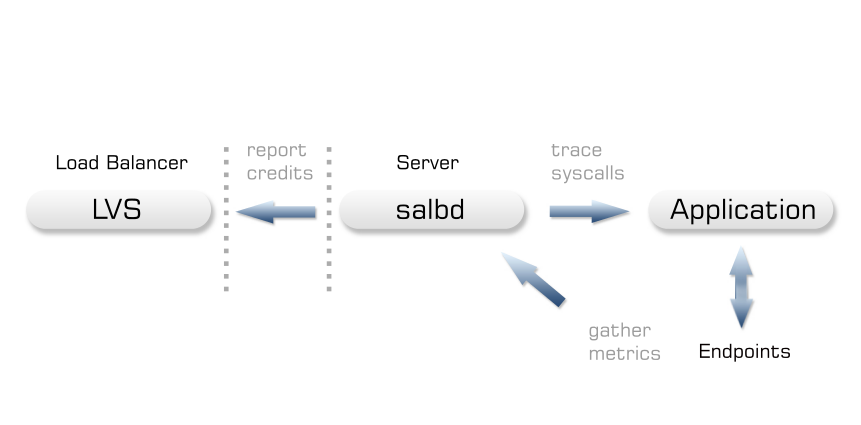
\includegraphics[width=\textwidth]{images/salbd-concept.png}
			\caption{Konzept von salbd (übernommen aus \cite{zinke2012})}
			\label{fig:salbd}
		\end{figure}
		
		% Auf dem Backend-Server dient salbd dazu
		% Backend-Servern dient dazu, durch entsprechende Metriken, die aktuelle Last des Servers zu
		% bestimmen. Aus diesen Werten wird anschließend eine Anzahl an Credits berechnet. Diese Credits
		% geben an wieviel Anfragen der Backend-Server zu diesem Zeitpunkt noch abarbeiten könnte ohne
		% überlastet zu sein. Dabei entspricht ein Credit einer Anfrage. Diese Credits werden dann von den
		% Backend-Servern an den Lastverteiler übermittelt. Der Lastverteiler wählt anschließend anhand
		% der gemeldeten Credits die Backend-Server aus. Dieses System ist in dem Sinne selbst-adaptiv,
		% dass Server deren Credits verbraucht sind und die keine neuen Credits melden, durch den
		% Lastverteiler ausgelassen werden.  Denn es ist davon auszugehen, dass der Server überlastet oder
		% ausgefallen ist. Sollte sich ein Server von einer Überlastsituation erholen und dem
		% Lastverteiler neue Credits übermitteln, wird dieser wieder in die Lastverteilung mit
		% aufgenommen.


		% Durch dieses Verfahren kann auf dem Lastverteiler ein einfacher Algorithmus wie Round-Robin
		% angewandt werden und es müssen keine Gewichte für die Verteilung bestimmt werden. Damit ist
		% dieses System durch seine eigene Anpassung besonders bei heterogenen Clustern geeignet.

		% Im Folgenden werden kurz die einzelnen Komponenten von salbnet vorgestellt.

	$~$\\

	In der Dissertation \cite{zinke2012} werden die Forschungsergebnisse über salbnet vorgestellt.
	Dabei ist die Idee von salbnet Credits zur Bewertung von Lastsitutationen zu nutzen. Das bedeutet,
	dass die Backend-Server ihre aktuelle Last ermitteln. Danach bestimmen die Backend-Server eine
	Credit-Anzahl, diese soll der Anzahl an Anfragen entsprechen, welche zum aktuellen Zeitpunkt
	zusätzlich vom Server abgearbeitet werden könnten. Diese Anzahl an Credits werden dem
	Lastverteiler gemeldet. Der Lastverteiler entscheidet dann per einfachen Round-Robin-Verfahren,
	welcher Server die nächste Anfrage erhält.  Dazu werden alle Server, welche noch Credits besitzen
	durchiteriert. Wird eine Anfrage einem Server zugewiesen, werden dessen Credits um eins
	verringert. Fallen die Credits eines Servers auf 0 und sendet der Server keine neuen Credits,
	fällt der Server aus der Liste der verfügbaren Server heraus. Meldet ein Server, dessen Credits
	bereits auf 0 gefallen waren, erneut Credits wird er wieder in die Verteilung mitaufgenommen. Die
	beiden wichtigsten Komponenten dieses Algorithmus sind die Metrik zur Berechnung der Credits und
	die Meldestrategie der Backend-Server.

	Die Metrik hat folgende Anforderungen zu erfüllen \cite{scsczile2008}:

	\begin{itemize}
		\item Sie sollte einfach zu berechnen sein.
		\item Sie sollte die aktuell zur Verfügung stehenden Ressourcen des Servers angeben.
		\item Sie sollte applikationsunabhängig sein.
		\item Sie sollte auch für Dienste mit mehreren Tausend Clients funktionieren.
	\end{itemize}

	Die Version von salbnet vor dieser Arbeit war auf TCP-Anfragen begrenzt. Dazu wurde eine Metrik
	beruhend auf der TCP-Backlog des Webservers entwickelt. Die Backlog erfüllt alle gestellten
	Anforderungen an eine gute Metrik. Sie ist einfach zu berechnen, da der aktuelle Füllstand und der
	maximale Füllstand leicht abfragbar sind. Die Backlog des Webservers entspricht einer
	Warteschlange für den Server. Solange die Backlog leer ist, kann der Webserver alle Anfragen sofort
	beantworten.  Sobald Anfragen in der Backlog gespeichert werden, ist der Server nicht mehr zu
	einer sofortigen Abarbeitung in der Lage, daher werden die wartenden Anfragen in der Backlog
	gespeichert. Das heißt, die Anzahl der noch freien Plätze in der Backlog gibt die Anzahl der noch
	möglichen Verbindungen an, bevor die Backlog voll ist. Wenn die Backlog voll ist und weitere
	Anfragen eintreffen, werden diese fallen gelassen. Somit kann die Anfrage nicht beantwortet
	werden.  Daher entspricht der aktuelle Füllstand der Backlog genau den aktuell zur Verfügung
	stehenden Ressourcen des Servers. Dadurch, dass die TCP-Backlog überwacht wird, ist diese Methode
	allgemein für alle Webserver nutzbar und somit applikationsunabhängig. Außerdem benötigt die
	Metrik keine besonderen Ressource, das heißt sie ist weder Speicher noch CPU-intensiv, und somit
	beeinflusst sie nicht die Leistung des Webservers. 

	Die Betrachtung der Backlog zeigt auch zwei wichtige Metriken zur Bewertung einer Lastverteilung
	für Webserver. Das Verwerfen einer Anfrage muss mit allen Möglichkeiten verhindert werden. Jede
	verworfene Anfrage kann einem verlorenen Nutzer oder Kunden entsprechen. Muss eine Anfrage sehr
	lange in der Backlog warten, ist dies zwar nicht so ungünstig, wie eine verworfene Anfrage, aber
	es bedeute eine längere Wartezeit für den Nutzer. Wenn dieser nicht bereit ist so lange auf eine
	Antwort zu warten, ist dies ebenfalls ein verlorener Nutzer oder Kunde. Das heißt eine gute
	Lastverteilung sollte zu einer geringen Zahl an verworfenen Anfragen und einer minimalen
	Antwortzeit führen.

	Als zweiter wichtiger Faktor des Credit-Ansatzes zählt neben der Metrik die Meldestrategie. Dabei
	ist es entscheident, wieviele und wie oft Credits gemeldet werden. Eine häufige Meldung von Credits
	könnte eine zusätzliche Last auf den Backend-Servern erzeugen. Werden Credits zu selten gemeldet
	kann es sein, dass der Backend-Server beim Lastverteiler aussortiert wird, weil seine Credits auf
	0 gefallen sind. Folgend werden 4 mögliche Meldestrategien vorgestellt \cite{scsczile2008,
	schneidenbach2009}.

	\paragraph{Plain} % {{{
	\label{par:plain}

		Plain stellt die einfachste Lösung vor. Dabei wird immer nach einem fixen Intervall die
		Differenz zwischen der maximalen Größe der Backlog und dem aktuellen Füllstand der Backlog
		gemeldet. Dies entspricht allen aktuell verfügbaren Ressourcen.

	% paragraph Plain }}}

	\paragraph{Soft + Hard Credits} % {{{
	\label{par:soft-hard-credits}

	Bei diesem Algorithmus werden dem Lastverteiler zweimal Credits mitgeteilt. Die Hard-Credits
	entsprechen den aktuell verfügbaren Ressourcen wie schon beim Plain-Algorithmus. Die Soft-Credits
	sind eine Empfehlung vom Backend-Server an den Lastverteiler. Sie ergeben sich aus den
	Hard-Credits und der aktuellen Lastsitutation, das heißt wenn der Server Probleme hat die Backlog
	abzuarbeiten sinken die Soft-Credits. Somit soll verhindert werden, dass zu viele Requests an den
	schon unter Last stehenden Server gesendet werden. Für den Lastverteiler sind grundsätzlich die
	Soft-Credits das ausschlaggebende Maß. Erst, wenn kein Server mehr über Soft-Credits verfügt
	werden die Hard-Credits beachtet.

	% paragraph Soft + Hard Credits }}}

	\paragraph{Dynamic Report} % {{{
	\label{par:dynamic-report}

	Dynamic Report ersetzt das feste Meldeintervall des vorherigen Algorithmus durch ein dynamisch
	berechnetes. Dabei bildet ein festes Intervall eine Untergrenze. Dies verhindert eine Meldung nach
	jeder abgearbeitet Anfrage. Dieser Algorithmus meldet oft Credits, wenn die Backlog nur leicht
	gefüllt ist und eine geringe Last	auf dem Server ist. Ist die Backlog stark gefüllt und der
	Server mit der Abarbeitung der Anfragen beschäftigt, werden die Credits seltener gemeldet. Das
	führt dazu, dass bei vielen Anfragen keine zusätzliche Last durch unnötige Credit-Meldungen entsteht
	und bei geringer Last der Lastverteiler immer aktuelle Werte vom Backend-Server besitzt.

	% paragraph Dynamic Report }}}

	\paragraph{Dynamic Pressure Relieve} % {{{
	\label{par:dynamic-pressure-relieve}

	Der Dynamic Pressure Relive Algorithmus kombiniert alle vorherigen Algorithmen. Es existieren
	wiederum Hard und Soft-Credits. Allerdings werden die Hard-Credits spätestens nach einem fixen
	Intervall gemeldet. Die Soft-Credits werden nach dem dynamischen Intervall aus dem Dynamic Report
	Algorithmus gemeldet. Allerdings werden falls die Soft-Credits gemeldet werden gleichzeitig auch
	die Hard-Credits gemeldet, da es eh schon zu einer Kommunikation zwischen Backend-Server und
	Lastverteiler kommt. Dieses Vorgehen soll verhindern, dass zu selten Hard-Credits bei hoher Last
	gemeldet werden und somit die Anzahl der Verworfenen Anfragen verringern.

	% paragraph Dynamic Pressure Relieve }}}
$~$\\

	Bei einer Simulation der verschiedenen Meldestrategien hat der Dynamic Pressure Relieve
	Algorithmus die besten Ergebnisse erzielt \cite{scsczile2008}.

	Um salbnet auf Webclustern zu testen, wurde der Benchmark servprep/servload \cite{habenschuss2011}
	entwickelt. Dabei ist servprep ein Programm, welches Logs des Apache Webservers einliest und diese
	modifizieren kann. So können alle Anfragen vervielfacht werden, Spitzenlasten verstärkt werden
	oder über einen Bewertungsalgorithmus neue Anfragen eingefügt werden, welche die Charakteristik
	des Log-Verlaufs nicht verändern. Die servload Anwendung ist der eigentliche Benchmark, welcher
	das von servprep vorbereitete Log wieder einspielt. Dabei ist servprep in der Programmiersprache
	Lua und servload in C geschrieben. In der weiteren Entwicklung des Benchmarks, wurde servprep in
	servload integriert. Dadurch konnte eine noch bessere Leistung erziehlt werden und der
	Ressourcenverbrauch minimiert werden. Im Rahmen einer Semesterarbeit \cite{menski2012} wurde
	servload in sofern erweitert, dass es Logs vom BIND DNS-Server verarbeiten und DNS-Anfragen über
	UDP versenden kann. Somit ist es möglich, servload in dieser Arbeit als Benchmark einzusetzen.

	In diesem Kapitel wurden die theoretischen Grundlagen und die bereits vorhandenen Metriken und
	Meldealgorithmen von salbnet erläutert. Basierend auf diesen Informationen wird im folgenden
	Kapitel ein Konzept erarbeitet, wie sich salbnet auf DNS-Anfragen anpassen lässt. Außerdem wurde
	ein Benchmark vorgestellt, welcher dazu geeignet ist die Erweiterung von salbnet auf seine
	Funktion zu testen und mit bestehenden Algorithmen zu vergleichen. 

	% chapter salbnet }}}

	\chapter{Konzept} % {{{
	\label{cha:konzept}

	In diesem Kapitel sollen mögliche Konzepte zur Erweiterung von salbnet für DNS-Anfragen
	vorgestellt werden. Danach wird eines der Konzepte ausgewählt und ein Entwurf zur Implementierung
	präsentiert. Die Implementierung des gewählten Entwurfs wird dann im Kapitel
	\ref{cha:implementierung} beschrieben.


		\section{Ansätze} % {{{
		\label{sec:ansaetze}

		Wie in Kapitel \ref{cha:salbnet} beschrieben, ist salbnet ursprünglich nur für TCP-Anwendungen
		konzipiert und für den Apache Webserver implementiert. Dazu wurde eine Metrik über die Backlog
		des TCP-Sockets des Webservers erstellt. Diese gibt konkret die Anzahl der Anfragen an, welche
		noch in der Backlog Platz finden würden. Das heißt, mehr als diese Anzahl an Anfragen sollten an
		den Server nicht gestellt werden, sonst existiert die Gefahr, dass die Anfragen verworfen
		werden. Aufgabe dieses Kapitels ist es verschiedene Ansätze zu beschrieben, welche eine ähnlich
		gute Metrik für UDP-Anfragen erzeugen. 

		\subsection*{Last-Metrik} % {{{

		Wenn sich ein Server in einer Überlastsitutation befindet, kann dies oft daran erkannt werden
		das bestimmte Ressourcen aufgebraucht sind. So kann eine 100\%ige CPU- oder RAM-Auslastung dafür
		sprechen, dass der Server an seine Grenzen gekommen ist. Daher wäre eine mögliche Metrik die
		Sammlung entsprechender Daten und ein anschließende Abschätzung bezüglich der verbleibenden
		Ressourcen.
		
		% subsection Last-Metrik }}}

		\subsection*{Verkehr-Metrik} % {{{

		Die Last eines Servers hängt von der Anzahl an einkommenden Anfragen und der Anzahl an
		abgearbeiteten (ausgehenden) Anfragen ab. Daher wäre es eine Möglichkeit alle eingehenden und
		ausgehenden Anfragen bzw. Antworten zu zählen. Anschließend kann abgeschätzt werden, ob der
		Server zur Zeit mehr Anfragen abarbeitet als ihn neue erreichen. Oder ob zu viele Anfragen
		eintreffen, welche er nicht mehr schnell genug abarbeiten kann.
		
		% subsection Verkehr-Metrik }}}

		\subsection*{Receive-Queue-Metrik} % {{{

		Ein Ansatz ähnlich des TCP-Ansatzes wäre es, die Receive-Queue des UDP-Sockets des DNS-Servers zu
		überwachen. Anders als beim TCP-Fall werden aber in der Receive-Queue keine Verbindungen
		verwaltet, sondern Pakete eingeordnet. Das heißt die Receive-Queue hat eine maximale Größe und
		ist bis zu einem bestimmten Punkt gefüllt. Dies sagt aber nichts über die Anzahl an Paketen in
		der Receive-Queue aus. Trotzdem könnte eine Metrik darin bestehen, den verbleibenden Platz in
		der Receive-Queue zu bestimmen. Und daraus eine Abschätzung zu treffen, wieviele weitere
		Anfragen aufgenommen werden könnten.

		% subsection Receive-Queue-Metrik }}}
		
		% section Ansätze }}}

		\section{Auswahl} % {{{
		\label{sec:auswahl}

		Nachdem mehrere Ansätze vorgestellt wurden, sollen diese nun bewertet werden. Danach wird ein
		Ansatz gewählt, welcher dann weiter verfeinert wird. Die Bewertung der Ansätze erfolgt nach den
		in Kapitel \ref{cha:salbnet} aufgeführten Anforderungen an eine Metrik:

		\begin{itemize}
			\item Sie sollte einfach zu berechnen sein.
			\item Sie sollte die aktuell zur Verfügung stehenden Ressourcen des Servers angeben.
			\item Sie sollte applikationsunabhängig sein.
			\item Sie sollte auch für Dienste mit mehreren Tausend Clients funktionieren.
		\end{itemize}

		\subsection*{Last-Metrik} % {{{

		Die Last-Metrik ist applikationsunabhängig und wird auch nicht durch die Anzahl der Clients
		beeinflusst. Jedoch ist es schwer aus den Faktoren wie der CPU-Last, RAM-Auslastung und Load
		eines Servers Aussagen über die noch zur Verfügung stehenden Ressourcen des Servers zu geben.
		Der Vergleich von CPU-Lasten ist vor allem in heterogenen Clustern schwer, dazu müsste eine
		Normalisierung durchgeführt werden, welche auf die entsprechenden Server ausgelegt ist. Daher
		ist diese Metrik nicht einfach zu berechnen und erfüllt die Anforderung nicht.

		Beweis: \cite{kunz1991} und \cite{lansch1994}
		% TODO: VS Buch und Paper einbauen

		% subsection Last-Metrik }}}

		\subsection*{Verkehr-Metrik} % {{{

		Die Verkehr-Metrik ist ebenfalls applikationsunabhängig und einfach zu berechnen. Es wird die
		Differenz der eingehenden und ausgehenden Anfragen ermittelt. Ist diese Differenz negativ, ist
		der Server schneller im Abarbeiten als das neue Anfragen eintreffen. Ist sie gleich 0 ist der
		Server in einem Gleichgewicht, in dem er alle eintreffenden Anfragen sofort beantworten kann.
		Ist die Differenz positiv stauen sich Anfragen beim Server. Steigt diese Differenz immer
		weiter an, kann davon ausgegangen werden, dass der Server Probleme hat weitere Anfragen
		abzuarbeiten. Die Probleme dieser Metrik sind jedoch die Abbildung der Differenz auf die
		verfügbaren Ressourcen des Servers. Das heißt, was sagen die eingehenden und ausgehenden Anfragen
		über die Anzahl der noch zusätzlich möglichen Anfragen aus. (????) Außerdem kann davon ausgegangen
		werden, dass ein Zählen aller ein- und ausgehenden Anfragen nicht gut skaliert. Das heißt, wenn
		eine hohe Anzahl an Anfragen auf den Server abgegeben werden, erzeugt das Überwachen aller
		Verbindungen eine zusätzliche Last. Daher erfüllt diese Metrik ebenfalls nicht die
		Anforderungen.
		
		% subsection Verkehr-Metrik }}}

		\subsection*{Receive-Queue-Metrik} % {{{

		Die Receive-Queue-Metrik ist, wie auch die beiden vorherigen, applikationsunabhängig. Sie
		erzeugt auch keine zusätzliche Last, wenn die Client-Anzahl ansteigt. Die Berechnung ist etwas
		schwieriger als beim TCP-Anwendungsfall, da wie bereits erwähnt, keine Verbindungen gespeichert
		werden, sondern Pakete. Allerdings kann aus dem verbleibenden Platz in der Receive-Queue und
		einer Abschätzung über die durchschnittliche Paketgröße eine Vorhersage getroffen werden, welche
		zusätzliche Anzahl an Anfragen der Server verarbeiten könnte. Damit erfüllt die Metrik auch die
		Anforderungen der einfachen Berechnung und der Angabe von verfügbaren Ressourcen.
		
		% subsection Receive-Queue-Metrik }}}

		Wie bereits durch die vorhergehenden Bewertung zu erkennen, hat nur die Receive-Queue-Metrik die
		Anforderung aus \cite{scsczile2008} an eine Metrik für salbnet erfüllt. Diese wird in Abschnitt
		\ref{sec:entwurf} genauer beschrieben und in Kapitel \ref{cha:implementierung} wird die
		konkrete Implementierung in salbnet erläutert.

		% section Auswahl }}}

		\section{Entwurf} % {{{ 
		\label{sec:entwurf}

		Die ausgewählte Metrik (Receive-Queue-Metrik) wird in diesem Abschnitt im Detail beschrieben.
		Dazu werden alle nötigen Messwerte identifiziert und eine Formel entwickelt, welche aus den
		Messwerten die Credits des Servers berechnen. Die Metrik soll den Server anhand der
		UDP-Receive-Queue des DNS-Servers bewerten. Daher werden folgende Messwerte benötigt: $~$\\
		
		\begin{tabular}{rl}
			$q_{max}$		  & die maximale Kapazität der UDP-Receive-Queue\\
			$q_{current}$ &	der aktuell belegte Speicherplatz in der UDP-Receive-Queue\\
			$p_{median}$  &	der Median der Paket-Größen in der UDP-Receive-Queue\\
		\end{tabular}
		
		$~$\\
		Mit Hilfe dieser Messwerte kann eine Abschätzung getroffen werden, wieviel weitere Pakete
		$p_{additional}$ (Anfragen) noch angenommen werden können, ohne dass eine Anfrage verworfen wird.
		Die Abschätzung ist in der Formel \ref{eq:additional} dargestellt. 

		\begin{equation}
			p_{additional} = \frac{q_{max} - q_{current}}{p_{median}}
			\label{eq:additional}
		\end{equation}

		Diese Abschätzung gibt eine Bewertung für den aktuellen Zeitpunkt an. Wie in Kapitel
		\ref{cha:salbnet} beschrieben existieren verschiedene Meldestrategie in salbnet. Bei den
		optimierten Strategien Dynamic Report und Dynamic Pressure Relieve werden die Credits in
		dynamisch berechneten Intervallen gemeldet. Das heißt zwischen zwei Credit-Meldungen kann sich
		die Receive-Queue stark verändern. Die Abschätzung enthält aber keinen Faktor, welcher die
		Tendenz seit der letzten Credit-Berechnung darstellt. Eine Lösung wäre, bei jeder Abarbeitung
		einer Anfrage Credits zu berechnen und diese zu speichern. Dadurch könnte der Verlauf mit in der
		Abschätzung genutzt werden. Allerdings würde dies besonders bei einer hohen Last auf dem Server
		zu einem zusätzlichen Aufwand führen, welcher die Leistung des Servers negativ beeinflussen
		kann. Als Kompromiss, zwischen ständiger Credit-Berechnung und Vernachlässigung des Verlaufs,
		gibt es die Möglichkeit nur auf Überlastsituationen zu reagieren. Das heißt es wird überprüft ob
		der Server sich zwischen zwei Credit-Meldungen in einer Überlastsitutation befunden hat. Dies
		kann zum Beispiel daran erkannt werden, ob Paket verworfen worden. Dies geschieht, wenn die
		maximale Kapazität der Receive-Queue erreicht wurde. Sind seit der letzten Credit-Meldung
		Anfragen verworfen wurden, sollte dies bei der Berechnung der aktuellen Credits beachtet werden.
		Dabei ist die Frage, wie das Verwerfen von Anfragen bewertet wird. In \cite{scsczile2008} wird
		eine nicht beantwortete Anfrage als ein verlorener Nutzer und potential als ein verlorener Kunde
		bewertet. Dabei ist zu beachten, dass die Aussage für den HTTP-Anwendungsfall getroffen wurde.
		Allerdings ist es auch bei DNS ein sinnvolles Ziel die verworfenen Anfragen zu minimieren. Daher
		sollen dem Lastverteiler 0 Credits gemeldet werden, wenn seit der letzten Credits-Meldung
		Anfragen verworfen wurde. Somit kann der Server die aktuellen Anfragen abarbeiten ohne weitere
		Anfragen zu erhalten. Dadurch wird sich die Last des Servers bis zur nächsten Credit-Meldung
		verringern. Anschließend können wieder Credits entsprechend der aktuellen Situation gemeldet
		werden.
		
		Wird nun die Anzahl der verworfenen Anfrage seit der letzten Credit-Meldung $p_{drop}$
		in der Abschätzung beachtet, ergibt sich Formel \ref{eq:credits} zur Berechnung der Credits des
		DNS-Servers.

		\begin{equation}
			Credits = \begin{cases}0 & p_{drop}>0\\ \frac{\displaystyle q_{max} - q_{current}}{\displaystyle p_{median}}
			  & \text{sonst}\end{cases}
			\label{eq:credits}
		\end{equation}


		% section Entwurf }}}

		\section{Fazit} % {{{
		\label{sec:konzept-fazit}
		
		% section Fazit }}}

	% chapter Konzept }}}

	\chapter{Implementierung} % {{{
	\label{cha:implementierung}

	% KERNEL 2.6.18 erwähnen; Vielleicht schonmal procfs einführen?

	Dieses Kapitel beschriebt die Implementierung der in Kapitel \ref{cha:konzept} entworfenen Metrik.
	Dazu wird in Abschnitt \ref{sec:anforderungen} die Frage geklärt, wie die in Abschnitt
	\ref{sec:entwurf} definierte Metrik berechnet wird. Das heißt, es wird gezeigt, welche
	Möglichkeiten existieren die benötigten Messwerte zu erhalten. Außerdem werden die erhaltenen
	Messwerte bewertet und es wird auf eventuelle Probleme oder Ungenauigkeiten dieser Werte
	eingegangen. Nachdem feststeht, wie alle Messwerte ermittelt werden können, wird in Abschnitt
	\ref{sec:erweiterung} auf die konkrete Implementierung in salbnet eingegangen. In Kapitel
	\ref{cha:messungen} werden Messungen vorgestellt, welche die erweiterte Version von salbnet mit
	einem Standard-Algorithmus vergleicht.
		
		\section{Anforderungen} % {{{
		\label{sec:anforderungen}

		In diesem Abschnitt sollen Möglichkeiten diskutiert werden, mit deren Hilfe die einzelnen
		Messwerte, für die in Abschnitt \ref{sec:entwurf} beschriebene Metrik, ermittelt werden können. Es
		werden dabei folgende Werte benötigt: $~$\\
		
		\begin{tabular}{rl}
			$q_{max}$		  & die maximale Kapazität der UDP-Receive-Queue\\
			$q_{current}$ &	der aktuell belegte Speicherplatz in der UDP-Receive-Queue\\
			$p_{median}$  &	der Median der Paket-Größen in der UDP-Receive-Queue\\
			$p_{drop}$    &	die Anzahl der verworfenen Pakete (Anfragen) seit der letzten Credit-Meldung\\
		\end{tabular}

		$~$\\
		\subsection*{Maximale Kapazität der UDP-Receive-Queue} % {{{

		\lstinputlisting[float,lastline=4,caption={Standard-Queue-Größe für UDP-Sockets},label=lst:default-queue]{listings/proc-rmem.txt}
		\lstinputlisting[float,firstline=6,caption={Erhöhen der Queue-Größe für UDP-Sockets},label=lst:test-queue]{listings/proc-rmem.txt}

		Die maximale Kapazität der UDP-Receive-Queue für jeden UDP-Socket wird im Kernel festgelegt. Der
		aktuelle Wert kann über das \texttt{/proc}-Dateisystem festgestellt werden. Beim
		\texttt{/proc}-Dateisystem \cite{benvenuti2005} handelt es sich um ein virtuelles Dateisystem,
		welches kernelinterne Datenstrukturen, in der Form von Dateien, in den Userspace exportiert. Im
		Listing \ref{lst:default-queue} sind die beiden entsprechenden Dateien im
		\texttt{/proc}-Dateisystem aufgeführt, welche die standard und maximale Größe der
		UDP-Receive-Queue eines UDP-Sockets bestimmen. Um diese Werte zu verändern, kann das Programm
		\texttt{sysctl} genutzt werden, welches Variablen im \texttt{/proc/sys}-Verzeichnis bearbeiten
		kann, oder es kann direkt in die entsprechenden Dateien ein neuer Wert geschrieben werden. Die
		Verwendung von \texttt{sysctl} ist in Listing \ref{lst:test-queue} zu sehen.
		% subsection Maximale Kapazität der UDP-Receive-Queue }}}

		\subsection*{Aktuell belegter Speicherplatz in der UDP-Receive-Queue} % {{{

		Der aktuell belegte Speicherplatz in der UDP-Receive-Queue eines UDP-Sockets kann ebenfalls über
		das \texttt{/proc}-Dateisystem ermittelt werden. Diese Information ist in der Datei
		\texttt{/proc/net/udp} enthalten. In Listing \ref{lst:proc-udp} ist ein Auszug aus dieser Datei
		zu sehen. Jede Zeile steht für einen Socket. Dabei ist \texttt{sl} der Hash-Slot des Sockets im
		Kernel. Die \texttt{local\_address} ist die lokale Adresse und Port des Sockets. Wenn der Socket
		direkt  mit einer entfernten Adresse verbunden ist, wird dies im Feld \texttt{rem\_address} angezeigt.
		Der Status des Sockets ist in \texttt{st} vermerkt und \texttt{tx\_queue} bzw.
		\texttt{rx\_queue} geben den Speicherverbrauch der UDP-Send-Queue bzw. UDP-Receive-Queue an. Es
		folgen noch weitere Werte, welche in diesem Zusammenhang unwichtig sind. Somit kann durch diese
		Datei der belegte Speicherplatz der UDP-Receive-Queue für einen bestimmten UDP-Socket ermittelt werden.

		Der Nachteil vom \texttt{/proc}-Dateisystem ist, dass bei wiederholten Abfragen eines Wertes,
		jedesmal eine Datei geöffnet, gelesen und geschlossen werden muss. Anschließend muss der Inhalt
		der Datei ausgewertet werden, um den gesuchten Wert zu finden. Eine möglicher Ersatz, vor allem
		bei der Netzwerkkonfiguration, bieten \texttt{Netlink}-Sockets \cite{rfc3549, gusowski2009}.
		Durch diese ist es möglich zwischen dem Kernel- und Userspace über einen Socket zu
		kommunizieren. Dies hat einige Vorteile gegenüber dem \texttt{/proc}-Dateisystem, da nur initial
		ein Socket erstellt werden muss, welche danach weiterverwendet werden kann, oder es können Werte
		gezielt abgefragt werden ohne sie aus einer Text-Repräsentation extrahieren zu müssen. In der
		Implementation von salbnet \cite{zinke2012,salbnet} wird ein \texttt{Netlink}-Socket genutzt um
		Informationen bezüglich der TCP-Backlog zu sammeln. Daher war es naheliegend ähnliches auch für
		die UDP-Receive-Queue anzuwenden. Allerdings ist das von salbnet verwendete Kernelmodul für den
		Kernel 2.6.18 entwickelt und kann nicht ohne Anpassungen mit neueren Kernel-Versionen genutzt
		werden. Die Erweiterung der \texttt{Netlink}-Sockets um ein UDP-Modul wurde jedoch erst im
		Kernel 3.3\cite{udpnetlink} aufgenommen. Somit ist die Verwendung eines \texttt{Netlink}-Sockets
		in salbnet für UDP nicht möglich.

		\lstinputlisting[float,caption={/proc/net/udp	Informationen zu UDP-Sockets},label=lst:proc-udp]{listings/proc-udp.txt}

		% subsection Aktuell belegter Speicherplatz in der UDP-Receive-Queue }}}

		\subsection*{Median der Paket-Größen in der UDP-Receive-Queue} % {{{

		Um den Median der Paket-Größen in der UDP-Receive-Queue bestimmen zu können, reicht der belegte
		Speicherplatz in der UDP-Receive-Queue nicht aus, denn es ist nich ermittelbar wieviele Pakete
		aktuelle in der Receive-Queue gespeichert sind. Wird jedoch ein Paket aus der Receive-Queue
		abgeholt, wird die Größe des Pakets zurückgeliefert. In Listing \ref{lst:strace} wurde das
		Programm \texttt{strace} genutzt, um die Systemcalls des BIND DNS-Servers nachzuvollziehen. In
		Zeile 12 ist zu erkennen, dass ein Paket vom BIND mit Hilfe der Funktion \texttt{recvmsg} aus
		der Queue abgeholt wird. Der Rückgabewert der Funktion gibt die Größe des Paketes in Byte an. In
		diesem Beispiel war das DNS-Paket 45 Byte groß. Somit ist es möglich den Funktions-Aufruf des
		BIND abzufangen und die Paket-Größe zu ermitteln.

		Allerdings ist die Größe des DNS-Paketes, wie sie von der Funktion \texttt{recvmsg}
		zurückgegeben wird, nicht der komplette Speicherbedarf des Pakets in der Receive-Queue. Im
		Linux-Kernel werden die Pakete, welche in einem Socket-Buffer liegen, mit Hilfe der
		Datenstruktur \texttt{sk\_buff} verwaltet. Im Anhang \ref{cha:skbuff} ist das Listing
		\ref{lst:skbuff} der \texttt{sk\_buff}-Datenstruktur für den Linux-Kernels 2.6.18 angeführt. Es ist
		zu erkennen, dass es eine große Anzahl an zusätzlichen Informationen in der Datenstruktur, neben
		dem eigentlichen DNS-Paket gespeichert, wird. Das Feld \texttt{truesize} in der Datenstruktur,
		enthält die vollständige Größe des Pakets in der Receive-Queue. Jedoch ist ein Zugriff auf
		diesen Wert aus dem Userspace nicht möglich.
		
		Um auf eine Anpassung im Kernelspace zu verzichten, wurde der Zusammenhang, zwischen der Größe
		des DNS-Pakets und dem Speicherplatz in der Receive-Queue, experimentell ermittelt. Hierzu
		wurden DNS-Pakete mit steigender Größe an einen BIND DNS-Server gesendet. Nach jedem Paket wurde
		der belegte Speicherplatz der Receive-Queue ermittelt und anschließend die Größe des Pakets mit
		der Funktion \texttt{recvmsg} ermittelt. Diese Versuche wurden mehrmals durchgeführt, dadurch
		konnte bestätigt werden, dass das Verhalten deterministisch ist und es einen direkt Zusammenhang
		zwischen der Größe des DNS-Pakets und dem benötigten Speicher in der Receive-Queue gibt. Der
		Header eines DNS-Pakets ist 12 Byte groß und die maximale Größe eines DNS-Pakets ist 512 Byte
		laut RFC \cite{rfc1035}, daher wurde das Experiment mit Paketen der Größe 12-576 Byte
		durchgeführt. Das Ergebnis ist in Tabelle \ref{tab:recvmsg} aufgeführt. Es zeigt sich, dass 376
		Byte die minimale Größe eines DNS-Pakets in der Receive-Queue ist. Überschreitet das DNS-Pakete
		eine Größe von 64 Byte wächst der Speicherbedarf um 128 Byte. Diese 128 Byte stehen
		ausschließlich für den Inhalt des DNS-Pakets zur Verfügung, da alle zusätzlichen Daten der
		\texttt{sk\_buff}-Datenstruktur bereits enthalten sind. Erhöht sich die Größe des DNS-Pakets
		ebenfalls um 128 Byte und überschreitet 192 Byte, wächst der Speicherbedarf wiederum um 128 Byte
		an. Zusammengefasst lässt sich sagen, dass ab einer Paket-Größe von 64 Byte alle 128 Byte eine
		Erhöhung des Speicherbedarfs um ebenfalls 128 Byte eintritt. Daher ist es möglich die Formel
		\ref{eq:recvmsg} zu bestimmen, welche anhand der Größe des DNS-Pakets (ermittelt durch
		\texttt{recvmsg}) den Speicherbedarf in der Receive-Queue berechnet. Es ist zu beachten, dass
		diese Formel nicht allgemeingültig ist und speziell für den Kernel 2.6.18 ermittelt wurde. Für
		andere Kernel-Versionen kann sich ein veränderter Zusammenhang ergeben und somit auch eine
		andere Formel gelten.		

		\begin{equation}
			\text{Receive-Queue} = \lfloor (\text{recvmsg} + 63) / 128 \rfloor * 128 + 376	
			\label{eq:recvmsg}
		\end{equation}

		\begin{table}
			\centering
			\begin{tabular}{|c|c|}\hline
				Receive-Queue & recvmsg \\\hline\hline
				376 & 12-64	\\
				504 & 65-192	\\
				632 & 193-320	\\
				760 & 321-448 \\
				888 &	449-576\\\hline
			\end{tabular}
			\caption{Experimentelle Bestimmung des Zusammenhangs zwischen der Größe des DNS-Pakets und dem
			Speicherplatz in der Receive-Queue (Angaben in Byte)}
			\label{tab:recvmsg}
		\end{table}

		\lstinputlisting[float,caption={strace-Ausgabe für den BIND-Server bei der Abfrage von
	\texttt{www.haiti.cs.uni-potsdam.de}},label=lst:strace]{listings/strace.txt}

		% subsection Median der Paket-Größen in der UDP-Receive-Queue }}}

		\subsection*{Verworfene Anfragen seit der letzten Credit-Meldung} % {{{

		In neueren Kernel-Versionen werden die Drops (Anzahl der verworfenen Anfragen) pro UDP-Socket
		ebenfalls in der Datei \texttt{/proc/net/udp} aufgeführt. Für die verwendete Kernel-Version
		2.6.18 gilt dies leider noch nicht. Daher wurde auf die Datei \texttt{/proc/net/snmp}
		zurückgegriffen. Wie in Listing \ref{lst:proc-snmp} zu sehen, wird in dieser Datei die Anzahl
		der systemweiten Drops als \texttt{InErrors} angegeben. Da in dieser Arbeit davon ausgegangen
		wird, dass es sich um ein DNS-Cluster handelt, welches ausschließlich zum Beantworten von
		DNS-Anfragen genutzt wird, kann davon	ausgegangen werden, dass der DNS-Server den Hauptanteil
		des UDP-Verkehrs erzeugt. Somit sind Drops, auch wenn diese nur systemweit angegeben werden,
		kritisch für den DNS-Server.
		
		\lstinputlisting[float,caption={/proc/net/snmp Protokoll-Information für SNMP-Programme},label=lst:proc-snmp]{listings/proc-snmp.txt}

		% subsection Verworfene Anfragen seit der letzten Credit-Meldung }}}

			
		% section Anforderungen }}}

		\section{Erweiterung von salbnet} % {{{
		\label{sec:erweiterung}

		\lstinputlisting[float,firstline=42,lastline=60,caption={Bestimmung der maximalen Kapzität der UDP-Receive-Queue (\texttt{linux/client\_metric.c} aus salbd)},label=lst:metric-max-udp]{listings/client_metric.c}
		\lstinputlisting[float,lastline=39,caption={Bestimmung des belegten Speicherplatz in der UDP-Receive-Queue (\texttt{linux/client\_metric.c} aus salbd)},label=lst:metric-udp-proc]{listings/client_metric.c}
		\lstinputlisting[float,firstline=63,caption={Bestimmung der verworfenen Anfragen (\texttt{linux/client\_metric.c} aus salbd)},label=lst:metric-drops-udp]{listings/client_metric.c}

		\lstinputlisting[float,lastline=38,caption={Bestimmung der Hard- und Soft-Credits	(\texttt{client\_report.c} aus salbd)},label=lst:metric-udp-proc]{listings/client_report.c}
		\lstinputlisting[float,firstline=40,caption={Bestimmung der maximalen und aktuellen Auslastung der UDP-Receive-Queue	(\texttt{client\_report.c} aus salbd)},label=lst:metric-drops-udp]{listings/client_report.c}

		\lstinputlisting[float,caption={Datenstruktur \texttt{nethook\_data} aus \texttt{nethook.h} der libnethook},label=lst:nethookh]{listings/nethook.h}

		\lstinputlisting[float,caption={Auszüge der Funktion \texttt{recvmsg} aus \texttt{nethook.c} der libnethook},label=lst:nethookc]{listings/nethook.c}
			
		% section Erweiterung von salbnet }}}

		\section{Fazit} % {{{
		\label{sec:implementierung-fazit}
		
		% section Fazit }}}

	% chapter Implementierung }}}

	\chapter{Messungen} % {{{
	\label{cha:messungen}

		In diesem Kapitel werden die durchgeführten Funktionsmessungen dargestellt. Es soll gezeigt
		werden, dass die Implementation funktionstüchtig und zum Verteilen von DNS-Anfragen geeignet
		ist. Außerdem wurde ein Vergleich zum Round-Robin-Verfahren des LVS durchgeführt. Dieser soll
		zeigen, dass das salbnet Verfahren eine bessere Verteilung der Last auf den Backend-Servern
		erzeugt. In Abschnitt \ref{sec:messumgebung} wird der Aufbau der Messumgebung erläutert. Danach
		wird in Abschnitt \ref{sec:messplan} der Ablauf der Messung beschrieben und in Abschnitt
		\ref{sec:auswertung} folgt eine Auswertung.

		\section{Messumgebung} % {{{
		\label{sec:messumgebung}

		Die Messumgebung soll ein realistisches Lastszenario wiederspiegeln. Dazu wurden aus dem
		IB-Cluster des Instituts für Informatik 4 Rechner ausgewählt (ib1, ib4, ib6, ib8). Die
		relevanten technischen Merkmale dieser Server sind in der Tabelle \ref{tab:netzwerkknoten}
		aufgeführt. Bei den	Maschinen ib1 und ib4 handelt es sich um baugleiche Server. Die Maschine ib6
		ist die älteste und auch schwächste Maschine, da sie nur einen Single-Core Prozessor besitzt.
		Der Aufbau soll ein DNS-Server-Cluster aus 3 Nameservern und einem Lastverteiler simulieren.
		Dabei ist die Maschine ib1 der Lastverteiler und die 3 heterogenen Maschinen ib4, ib6 und ib8
		stellen jeweils einen BIND Nameserver bereit.	Auf allen ib-Maschinen ist ein CentOS 5.7 mit dem
		Kernel 2.6.18-274.12.1.el5 installiert.  Auf den Maschinen ib4, ib6 und ib8 ist BIND in der
		Version 9.3.6-20.P1 installiert. Auf den BIND Servern wurde die
		\texttt{haiti.cs.uni-potsdam.de}-Domain mit dem Stand vom 26. Oktober 2011 eingerichtet. Die
		Anzahl der einzelnen Resource Record Typen ist in Tabelle \ref{tab:rr-domain} aufgeführt. Die
		Konfiguration des BIND Servers ist in Anhang \ref{lst:bind-conf} zu finden. Um eine höhere
		Auslastung der Nameserver zu erhalten wurde die UDP-Receive-Queue auf den Maschinen ib1, ib4,
		ib6 und ib8 auf \unit[24]{MB} erhöht. Dadurch wird verhindert, das DNS-Anfragen verworfen
		werden, weil die Receive-Queue voll ist, obwohl der Nameserver diese noch beantworten könnte.
		
		Zum Absenden der DNS-Anfragen wird die Maschine node015 aus dem Leibniz-Cluster des Institut für
		Informatik genutzt. Sie besitzt einen Quad-Core Prozessor und 12 GB RAM (siehe Tabelle
		\ref{tab:netzwerkknoten}). Auf ihr wird der servload Benchmark ausgeführt, da dieser eine
		ausreichend hohe Last erzeugen muss um die 3 Nameserver zu belasten ist diese leistungsstarke
		Maschine notwendig.

		\begin{table}
			\centering
			\begin{tabular}{|c|c|c|c|c|l|}\hline
				Node & CPU &  Taktung & Kerne & RAM & Funktion \\\hline\hline
				node015 & Intel Xeon E5520 & \unit[2,27]{GHz} & 1 $\times$ 4 & \unit[12]{GB} & servload\\
				ib1 & AMD Opteron 244 & \unit[1,8]{GHz} & 2 $\times$ 1 & \unit[4]{GB} & LVS, salbd (Server)\\
				ib4 & AMD Opteron 244 & \unit[1,8]{GHz} & 2 $\times$ 1 & \unit[4]{GB} & BIND, salbd (Client)\\
				ib6 & Intel Pentium 4 & \unit[2,8]{GHz} & 1 $\times$ 1 & \unit[4]{GB} & BIND, salbd (Client)\\
				ib8 & Intel Xeon 3040 & \unit[1,86]{GHz} & 1 $\times$ 2 & \unit[4]{GB} & BIND, salbd (Client)\\\hline
			\end{tabular}
			\caption{Technische Daten der verwendeten Netzwerkknoten}
			\label{tab:netzwerkknoten}
		\end{table}

		\begin{table}
			\centering
			\begin{tabular}{|c|c|}\hline
				Resource Record & Anzahl \\\hline\hline
				A & 107 \\
				NS & 4 \\
				MX & 2 \\
				CNAME & 2 \\
				PTR & 106 \\
				SOA & 1 \\\hline
			\end{tabular}
			\caption{Anzahl der Resource Record Typen in der \texttt{haiti.cs.uni-potsdam.de}-Domain}
			\label{tab:rr-domain}
		\end{table}
			
		% section Messumgebung }}}

		\section{Messplan} % {{{
		\label{sec:messplan}

		Zur Durchführung der  Messung wurde ein anonymisiertes Log des authorativen Nameservers der
		\texttt{haiti.cs.uni-potsdam.de}-Domain verwendet. Das Log enthält den Zeitraum von 10:41 am 27.
		September 2011 bis 6:25 am 2. Oktober 2011. Über den Zeitraum von 6944 Minuten enthält das Log
		1003149 Anfragen, welche hauptsächlich Anfragen nach \texttt{A} und \texttt{AAAA} Resource
		Records sind (siehe Tabelle \ref{tab:log}). Es enthält 1026 Sessions, wobei eine Session als
		alle Anfragen eines einzelnen Users definiert ist. Dadurch ergeben sich die Verhältnisse von
		\unit[9,33]{\nicefrac{Anfragen}{Sekunde}} und \unit[977,63]{\nicefrac{Anfragen}{Session}}. Diese
		Last würde keinen der 3 Nameserver auslasten. Um eine höhere Last erzeugen zu können wurde ein
		Zeitabschnitt um das Maximum des Logs ausgewählt. Dieser wurde dann durch die
		\texttt{multiply}-Methode des servload Benchmarks verstärkt um eine ausreichend hohe Last zu
		erzeugen. Als Zeitraum wurden 5 Minuten von 5:55 bis 6:00 am 29. September 2011 gewählt, in
		diesem liegt das Maximum mit \unit[204]{\nicefrac{Anfragen}{Sekunde}}. In diesem Intervall
		werden 22.594 Anfragen von 33 Sessions gestellt. Der sehr kurze Zeitraum von 5 Minuten war
		notwendig, um durch eine hohe Verstärkung das Nameserver-Cluster auszulasten. Wäre ein
		längerer Zeitraum gewählt worden, hätte der Arbeitspeicher des node015 Rechners nicht
		ausgereicht um das komplette verstärkte Log vorzuhalten.
		
		Mit dem ausgewählten Intervall wurden jeweils 3 Messungen mit unterschiedlichen
		Multiplikationsfaktoren durchgeführt. Es wurden die Faktoren 400, 800 und 1600 gewählt um hohe
		Lastsitutationen zu erzeugen. Die daraus resultierende Anzahl an Anfragen, Sessions und
		\nicefrac{Anfragen}{Sekunde} sind in der Tabelle \ref{tab:multiply} zu sehen. Eine höhere
		Verstärkung war wiederum nicht möglich ohne an die Grenzen des Arbeitsspeicher zu stoßen.

		Verglichen wurden der gewichtete Round-Robin-Algorithmus des LVS mit dem dynamic pressure
		relieve salbd Algorithmus. Die Gewichte für den Round-Robin Algorithmus wurden mit Hilfe des
		Benchmarks UnixBench \cite{unixbench} bestimmt. Dieser
		Benchmark führt verschieden Tests aus und ermitteln eine Gesamtbewertung des Systems. Die
		Messergebnisse für die Machinen ib4, ib6 und ib8 sind im Anhang \ref{lst:unixbench} zu sehen. Es
		wurden die Werte 788, 623 und 1180 für die ib4, ib6 und ib8 bestimmt. Diese Gewichte haben sich
		bereits in anderen Messungen als sinnvoll für den Round-Robin-Algorithmus erwiesen, deshalb
		wurden bei diesen Messungen wiederum auf sie zurückgegriffen. Bei dem salbd Algorithmus müssen
		keine Gewichte angegeben werden. Allerdings muss eine Meldestrategie gewählt werden. Messungen
		in einem TCP-Szenario haben den Algorithmus dynamic pressure relieve als eine der besten
		Meldestrategien ermittelt. Deshalb wurde auch in diesem DNS-Szenario dieser ausgewählt. Die
		Credits werden von den Backend-Servern über TCP zum Lastverteiler übermittelt. Die salbd
		Konfiguration für den Lastverteiler (ib1) ist in Anhang \ref{lst:salbd-server} und die
		Konfigurationen für salbd auf den Backend-Servern (ib4, ib6 und ib8) ist in Anhang
		\ref{lst:salbd-client} und \ref{lst:salbd-bind} angeführt.  Jede Messung wurde 51 mal
		wiederholt, da die Messwerte stark schwanken. Somit wurden 306 Messungen durchgeführt

		\begin{table}
			\centering
			\begin{tabular}{|c|cc|}\hline
				Anfragen & 1003149 & \\
				Sessions & 1026 & \\
				\nicefrac{Anfragen}{Sekunde} & 9,33 &\\
				\nicefrac{Anfragen}{Session} & 977,73 &\\
				A & 327861 & \unit[32,68]{\%}\\
				AAAA & 609821 & \unit[60,79]{\%}\\
				NS & 3575 & \unit[0,36]{\%}\\
				MX & 669 & \unit[0,07]{\%}\\
				PTR & 60553 & \unit[6,04]{\%} \\ \hline
			\end{tabular}
			\caption{Analyse des BIND Logs der \texttt{haiti.cs.uni-potsdam.de}-Domain}
			\label{tab:log}
		\end{table}

		\begin{figure}
			\centering
			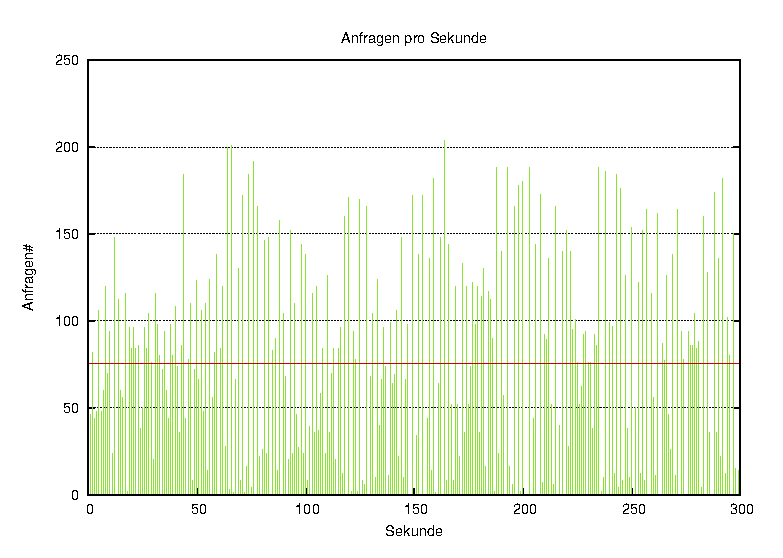
\includegraphics[width=\textwidth]{plots/requests}
			\caption{Anfragen pro Sekunden für das Log vom 29. September 2011 von 5:55 bis 6:00}
			\label{fig:requests}
		\end{figure}

		\begin{table}
			\centering
			\begin{tabular}{|lrrrr|}\hline
				Faktor & Anfragen & Sessions & $\varnothing$ \nicefrac{Anfragen}{Sekunde} &
				maximale \nicefrac{Anfragen}{Sekunde} \\\hline\hline
				1 & 22.594 & 33 & 75,31 & 204 \\
				400 & 9.037.600 & 13.200 & 30.125,33 & 81.600 \\
				800 & 18.075.200 & 26.400 & 60.250,67 & 163.200 \\
				1600 & 36.150.400 & 52.800 & 120.501,33 & 326.400 \\\hline
			\end{tabular}
			\caption{Kennzahlen des modifizierten Log Intervalls}
			\label{tab:multiply}
		\end{table}


		% section Messplan }}}

		\section{Auswertung} % {{{
		\label{sec:auswertung}

		Um die Messungen auszuwerten wurden während der Messungen minütlich die Werte der aktuellen CPU
		und Memory-Auslastung sowie der Load-Wert der Maschinene ib1, ib4, ib6 und ib8 abgefragt. Dies
		wurde mit Hilfe von \texttt{net-snmp}\ durchgeführt. Außerdem wurden die Ausgaben vom servload
		Benchmark gespeichert. 
			
		% section Auswertung }}}

		\section{Fazit} % {{{
		\label{sec:messungen-fazit}
		
		% section Fazit }}}

	% chapter Messungen }}}

	\chapter{Zusammenfassung und Ausblick} % {{{
	\label{cha:zusammenfassung}

		\section{Zusammenfassung} % {{{
		\label{sec:zusammenfassung}
			
		% section Zusammenfassung }}}

		\section{Ausblick} % {{{
		\label{sec:ausblick}

		Metrik funktioniert, aber:
		\begin{itemize}
			\item Ist sie zu optimistisch?
			\item vielleicht eher abschätzung über Größe des bis jetzt größten Pakets
			\item Kann man diese Kernel spezifische Magic allgemeiner machen
			\item Ist es den aufwand Wert den exakten Verlauf zwischen 2 Meldungen zu betrachten und ein
				Tendenz mit in die Berechnung der Credits mit einfließen zu lassen
		\end{itemize}
		
		% section Ausblick }}}

	% chapter Zusammenfassung }}}

	% Mainmatter }}}

	% Appendix {{{ 
	\appendix

	\chapter{Messumgebung} % {{{ 
	\label{cha:messumgebung}

	\lstinputlisting[language=sh,caption={salbd Konfiguration für ib1	(LVS)},label=lst:salbd-server]{listings/salbd.conf.server}

	\lstinputlisting[language=sh,caption={salbd Konfiguration für ib4, ib6 und ib8 (BIND)},label=lst:salbd-client]{listings/salbd.conf.client}

	\lstinputlisting[language=sh,caption={salbd BIND Konfiguration für ib4, ib6 und	ib8},label=lst:salbd-bind]{listings/salbd.networks.conf.client}

	\lstinputlisting[language=sh,caption={BIND Konfiguration für ib4, ib6 und ib8},label=lst:bind-conf]{listings/named.conf}

	\lstinputlisting[language=,breaklines=true,numbers=none,caption={UnixBench Resultate für die Maschinen ib4, ib6 und
	ib8},label=lst:unixbench]{listings/result_unixbench.dat}

	% chapter Messumgebung }}}

	\chapter{sk\_buff} % {{{
	\label{cha:skbuff}

	\lstinputlisting[language=C,firstline=193,lastline=304,caption={\texttt{sk\_buff}-Datenstruktur in der Datei
	\texttt{skbuff.h} vom Linux-Kernel 2.6.18},label=lst:skbuff]{listings/skbuff.h}

	% chapter skbuff }}}

	% Appendix }}}

	% Backmatter {{{
	\backmatter
	\pagenumbering{Roman}

	\listoffigures{}
	\listoftables{}

	% Bibliography {{{
	% \nocite{*}
	\bibliographystyle{dinat}
	\bibliography{references}
	% }}}

	% Backmatter }}}

\end{document}
